\documentclass[oneside,14pt]{extarticle}
\usepackage{cmap}
\usepackage[utf8]{inputenc}
\usepackage[english,ukrainian]{babel}
\usepackage{graphicx}
\usepackage{geometry}
\usepackage{listings}
\usepackage{multicol}
\usepackage{float}
\usepackage{amsmath}
\usepackage{subfig}
\geometry{
	a4paper,
	left=20mm,
	right=20mm,
	top=15mm,
	bottom=15mm,
}
\lstset{
	language=c,
	tabsize=4,
	keepspaces,
	showstringspaces=false,
	frame=single,
	language=C,
	breaklines,
}
\graphicspath{ {./pictures} }
\setlength{\parindent}{4em}

\newcommand\subject{Основи програмування вбудованих систем}
\newcommand\lecturer{старший викладач кафедри ПЗ\\Кутельмах Р.К.}
\newcommand\teacher{старший викладач кафедри ПЗ\\Кутельмах Р.К.}
\newcommand\mygroup{ПЗ-32}
\newcommand\lab{2}
\newcommand\theme{Програмна реалізація мобільного застосунку}
\newcommand\purpose{Розробити мобільний застосунок згідно з обраним варіантом}

\begin{document}
\begin{normalsize}
	\begin{titlepage}
		\thispagestyle{empty}
		\begin{center}
			\textbf{МІНІСТЕРСТВО ОСВІТИ І НАУКИ УКРАЇНИ\\
				НАЦІОНАЛЬНИЙ УНІВЕРСИТЕТ "ЛЬВІВСЬКА ПОЛІТЕХНІКА"}
		\end{center}
		\begin{flushright}
			\textbf{ІКНІ}\\
			Кафедра \textbf{ПЗ}
		\end{flushright}
		\vspace{80pt}
		\begin{center}
			\textbf{ЗВІТ}\\
			\vspace{10pt}
			до лабораторної роботи № \lab\\
			\textbf{на тему}: <<\textit{\theme}>>\\
			\textbf{з дисципліни}: <<\subject>>
		\end{center}
		\vspace{80pt}
		\begin{flushright}
			
			\textbf{Лектор}:\\
			\lecturer\\
			\vspace{28pt}
			\textbf{Виконав}:\\
			
			студент групи \mygroup\\
			Коваленко Д.М.\\
			\vspace{28pt}
			\textbf{Прийняв}:\\
			
			\teacher\\
			
			\vspace{28pt}
			«\rule{1cm}{0.15mm}» \rule{1.5cm}{0.15mm} 2024 р.\\
			$\sum$ = \rule{1cm}{0.15mm}……………\\
			
		\end{flushright}
		\vspace{\fill}
		\begin{center}
			\textbf{Львів — 2024}
		\end{center}
	\end{titlepage}
		
	\begin{description}
		\item[Тема.] \theme.
		\item[Мета.] \purpose.
	\end{description}


	\section*{Хід роботи}
	\section*{Теоретичні відомості}
	Flutter - це відкрите програмне забезпечення для створення мобільних, веб- та настільних програм з одного коду, розроблене компанією Google. Основним концептом Flutter є використання одного мовного коду для розробки для різних платформ, що дозволяє розробникам ефективно створювати крос-платформенні додатки.
	
	\begin{itemize}
		\item У Flutter все є віджетом - від простого тексту або кнопки до складних макетів та анімацій. Віджет - це будівельний блок інтерфейсу користувача, який складається з атрибутів, що визначають його вигляд і поведінку.
		\item Flutter дозволяє розробникам створювати додатки для різних платформ, таких як Android, iOS, веб та настільні (за допомогою проекту Flutter Desktop) з використанням єдиного кодової бази.
		\item Мова програмування, що використовується у Flutter, називається Dart. Dart - це ефективна, компільована мова зі строгим типізацією, яка використовується для розробки додатків у Flutter. Вона має сучасний синтаксис, який допомагає розробникам писати більш безпечний та швидкий код.
		\item Hot Reload: Це одна з ключових функцій Flutter, яка дозволяє розробникам швидко бачити зміни, зроблені в коді, на відразу на емуляторі або фізичному пристрої без необхідності перезапуску всього додатку.
		\item Flutter використовує власний движок малювання, що дозволяє досягнути високої продуктивності та плавності анімацій навіть на простих пристроях.
		\item Flutter надає розробникам гнучкість та контроль над виглядом і поведінкою додатків, дозволяючи легко налаштовувати різні аспекти інтерфейсу користувача.
		\item У Flutter активна спільнота розробників, яка постійно розвивається та надає підтримку через форуми, чати, документацію та інші ресурси.
	\end{itemize}
	Flutter є потужним інструментом для розробки крос-платформенних додатків, який надає розробникам широкі можливості для створення ефективних, привабливих та швидких додатків для різних платформ.
	
	\section*{Опис основних класів}
	
	\begin{itemize}
		\item \textit{models/note.dart} - Модель нотатки для роботи з базою даних.
		\item \textit{pages/} \begin{itemize}
			\item \textit{pages/archived\_notes.dart} - сторінка для відображення архівованих нотаток.
			\item \textit{pages/deleted\_notes.dart} - сторінка для відображення видалених нотаток.
			\item \textit{pages/edit\_note.dart} - сторінка для редагування та створення нотаток.
			\item \textit{pages/home.dart} - головна сторінка.
			\item \textit{pages/options.dart} - сторінка налаштувань додатку.
			\item \textit{pages/privacy.dart} - сторінка з описом умов використання додатку.
		\end{itemize}
		\item \textit{services/} \begin{itemize}
			\item \textit{services/firebase\_auth.dart} - сервіс для взаємодії з авторизацією користувачів.
			\item \textit{services/google\_calendar.dart} - сервіс для взаємодії з Google Calendar.
		\end{itemize}
		\item \textit{widgets/} \begin{itemize}
			\item \textit{widgets/bool\_dialog.dart} - віджет для відображення діалогу.
			\item \textit{widgets/calendar.dart} - віджет календаря.
			\item \textit{widgets/note\_preview.dart} - віджет для відображення нотатки.
			\item \textit{widgets/note\_preview\_list.dart} - віджет для відображення списку нотаток.
			\item \textit{widgets/snack\_bar.dart} - віджет для відображення повідомлень.
			\item \textit{widgets/upcoming\_notes\_list.dart} - віджет для відображення списку найближчих подій.
		\end{itemize}
	\end{itemize}
	
	\section*{Код програми}
	{\small
		\begin{lstlisting}
import 'package:flutter/material.dart';
import 'package:lab/Pages/archived_notes.dart';
import 'package:lab/Pages/deleted_notes.dart';
import 'package:lab/Pages/edit_note.dart';
import 'package:lab/Pages/privacy.dart';
import 'package:lab/Pages/options.dart';
import 'package:lab/Models/note.dart';
import 'package:lab/Services/firebase_auth.dart';
import 'package:lab/Services/google_calendar.dart';
import 'package:lab/Widgets/calendar.dart';
import 'package:lab/Widgets/note_preview_list.dart';
import 'package:lab/Widgets/snack_bar.dart';

class HomePage extends StatefulWidget {
	const HomePage({super.key});
	
	@override
	State<HomePage> createState() => _HomePageState();
}

class _HomePageState extends State<HomePage> {
	final GlobalKey<ScaffoldState> scaffoldKey = GlobalKey<ScaffoldState>();
	late List<Note> notes;
	bool isLoading = true;
	
	@override
	void initState() {
		super.initState();
		DatabaseHelper.instance.fetchNotes().then((result) {
			setState(() {
				notes = result;
				isLoading = false;
			});
		});
	}
	
	@override
	Widget build(BuildContext context) {
		if (isLoading) {
			return const LinearProgressIndicator();
		}
		
		return Scaffold(
		key: scaffoldKey,
		appBar: _topBar(),
		body: _body(),
		bottomNavigationBar: _bottomBar(),
		drawer: _leftDrawer(),
		endDrawer: Auth.isLoggedIn ? _rightDrawer() : null,
		floatingActionButton: _addButton(),
		resizeToAvoidBottomInset: false,
		);
	}
	
	PreferredSizeWidget _topBar() {
		return AppBar(
		backgroundColor: Theme.of(context).colorScheme.inversePrimary,
		centerTitle: true,
		toolbarHeight: 80,
		leading: IconButton(
		icon: const Icon(
		Icons.menu,
		size: 25,
		),
		onPressed: () {
			scaffoldKey.currentState?.openDrawer();
		}),
		actions: [
		IconButton(
		icon: Auth.userIcon,
		onPressed: () async {
			if (Auth.isLoggedIn) {
				scaffoldKey.currentState?.openEndDrawer();
			} else {
				try {
					await Auth.signInWithGoogle();
					setState(() {});
				} catch (e) {
					if (mounted) {
						snackBar(context, e.toString(), durationSec: 10);
					}}}}),],);
	}
	
	Widget _body() {
		filter(e) => !e.isArchived && !e.isDeleted;
		
		return NotePreviewList(
		notes: notes,
		filter: filter,
		orElse: "Press the button to create a note.");
	}
	
	Widget _bottomBar() {
		void openFullCalendar() => showModalBottomSheet<void>(
		context: context,
		isScrollControlled: true,
		builder: (BuildContext context) {
			return Calendar.full(context, notes);
		},
		);
		
		return GestureDetector(
		behavior: HitTestBehavior.opaque,
		onVerticalDragUpdate: (details) {
			if (details.delta.dy < 0) {
				openFullCalendar();
			}
		},
		child: BottomAppBar(
		height: 190,
		child:
		Column(mainAxisAlignment: MainAxisAlignment.start, children: [
		IconButton(
		icon: const Icon(Icons.arrow_upward),
		onPressed: () => openFullCalendar()),
		Calendar.preview(notes),
		])));
	}
	
	Widget _leftDrawer() {
		return Drawer(
		child: ListView(
		padding: EdgeInsets.zero,
		children: [
		DrawerHeader(
		decoration: BoxDecoration(
		color: Theme.of(context).colorScheme.secondary,
		),
		child: Text(
		'Lab',
		style: TextStyle(
		color: Theme.of(context).colorScheme.onSecondary,
		fontSize: 24,),),),
		ListTile(
		leading: const Icon(Icons.settings),
		title: const Text('Options'),
		onTap: () {
			Navigator.pop(context);
			Navigator.of(context).push(
			MaterialPageRoute(builder: (ctx) => const OptionsPage()));
		},
		),
		ListTile(
		leading: const Icon(Icons.archive),
		title: const Text('Archived'),
		onTap: () async {
			Navigator.pop(context);
			await Navigator.push(
			context,
			MaterialPageRoute(
			builder: (ctx) => ArchivedNotesPage(notes: notes)),
			);
			// Trigger redraw.
			setState(() {});
		},
		),
		ListTile(
		leading: const Icon(Icons.delete),
		title: const Text('Deleted'),
		onTap: () async {
			Navigator.pop(context);
			await Navigator.push(
			context,
			MaterialPageRoute(
			builder: (ctx) => DeletedNotesPage(notes: notes)),
			);
			// Trigger redraw.
			setState(() {});
		},
		),
		if (false)
		ListTile(
		leading: const Icon(Icons.help),
		title: const Text('Help'),
		onTap: () async {
			// TODO: Open Help.
			Navigator.pop(context);
			await DatabaseHelper.instance.deleteAllNotes();
			setState(() {
				notes.clear();
			});
		},
		),
		ListTile(
		leading: const Icon(Icons.info),
		title: const Text('About'),
		onTap: () {
			Navigator.pop(context);
			showAboutDialog(context: context);
		},),],),);
	}
	
	Widget _rightDrawer() {
		return Drawer(
		child: ListView(
		padding: EdgeInsets.zero,
		children: [
		DrawerHeader(
		decoration: BoxDecoration(
		color: Theme.of(context).colorScheme.secondary,
		),
		child: Text(
		Auth.userName!,
		style: TextStyle(
		color: Theme.of(context).colorScheme.onSecondary,
		fontSize: 24,
		),
		),
		),
		if (false)
		ListTile(
		leading: const Icon(Icons.account_box),
		title: const Text('Account'),
		onTap: () {
			// TODO: Open account.
			Navigator.pop(context);
		},
		),
		ListTile(
		leading: const Icon(Icons.sync),
		title: const Text('Sync'),
		onTap: () async {
			Navigator.pop(context);
			try {
				List<Note> result = (await GoogleCalendar.load())
				.where((gn) => !notes.any((n) => gn.googleId == n.googleId))
				.toList();
				await DatabaseHelper.instance.insertNotes(result);
				setState(() {
					notes.addAll(result);
				});
			} catch (e) {
				if (mounted) {
					snackBar(context, e.toString(), durationSec: 10);
				}
			}
		},
		),
		ListTile(
		leading: const Icon(Icons.logout),
		title: const Text('Log out'),
		onTap: () async {
			try {
				await Auth.signOutFromGoogle();
				setState(() {});
			} catch (e) {
				if (mounted) {
					snackBar(context, e.toString(), durationSec: 10);
				}
			}
			if (mounted) {
				Navigator.pop(context);
			}
		},
		),
		ListTile(
		leading: const Icon(Icons.privacy_tip),
		title: const Text('Privacy'),
		onTap: () async {
			Navigator.pop(context);
			Navigator.of(context).push(
			MaterialPageRoute(builder: (ctx) => const PrivacyPage()));
		},),],),);
	}
	
	Widget _addButton() {
		return FloatingActionButton(
		onPressed: () async {
			Note result = await Navigator.push(
			context,
			MaterialPageRoute(builder: (ctx) => EditNotePage(note: Note())),
			);
			if (!result.isEmpty()) {
				if (notes.any((note) => note.id == result.id)) {
					await DatabaseHelper.instance.updateNote(result);
					setState(() {
						int index = notes.indexWhere((note) => note.id == result.id);
						if (index != -1) {
							notes[index] = result;
						}
					});
				} else {
					await DatabaseHelper.instance.insertNote(result);
					setState(() {
						notes.add(result);
					});
				}
			} else {
				if (notes.any((note) => note.id == result.id)) {
					await DatabaseHelper.instance.deleteNote(result);
					setState(() {
						notes.removeWhere((note) => note.id == result.id);
					});
				}
			}
		},
		child: const Icon(Icons.add),
		);
	}
}
		\end{lstlisting}
	}
	
	\begin{figure}[H]
		\begin{minipage}{0.48\textwidth}
			\centering
			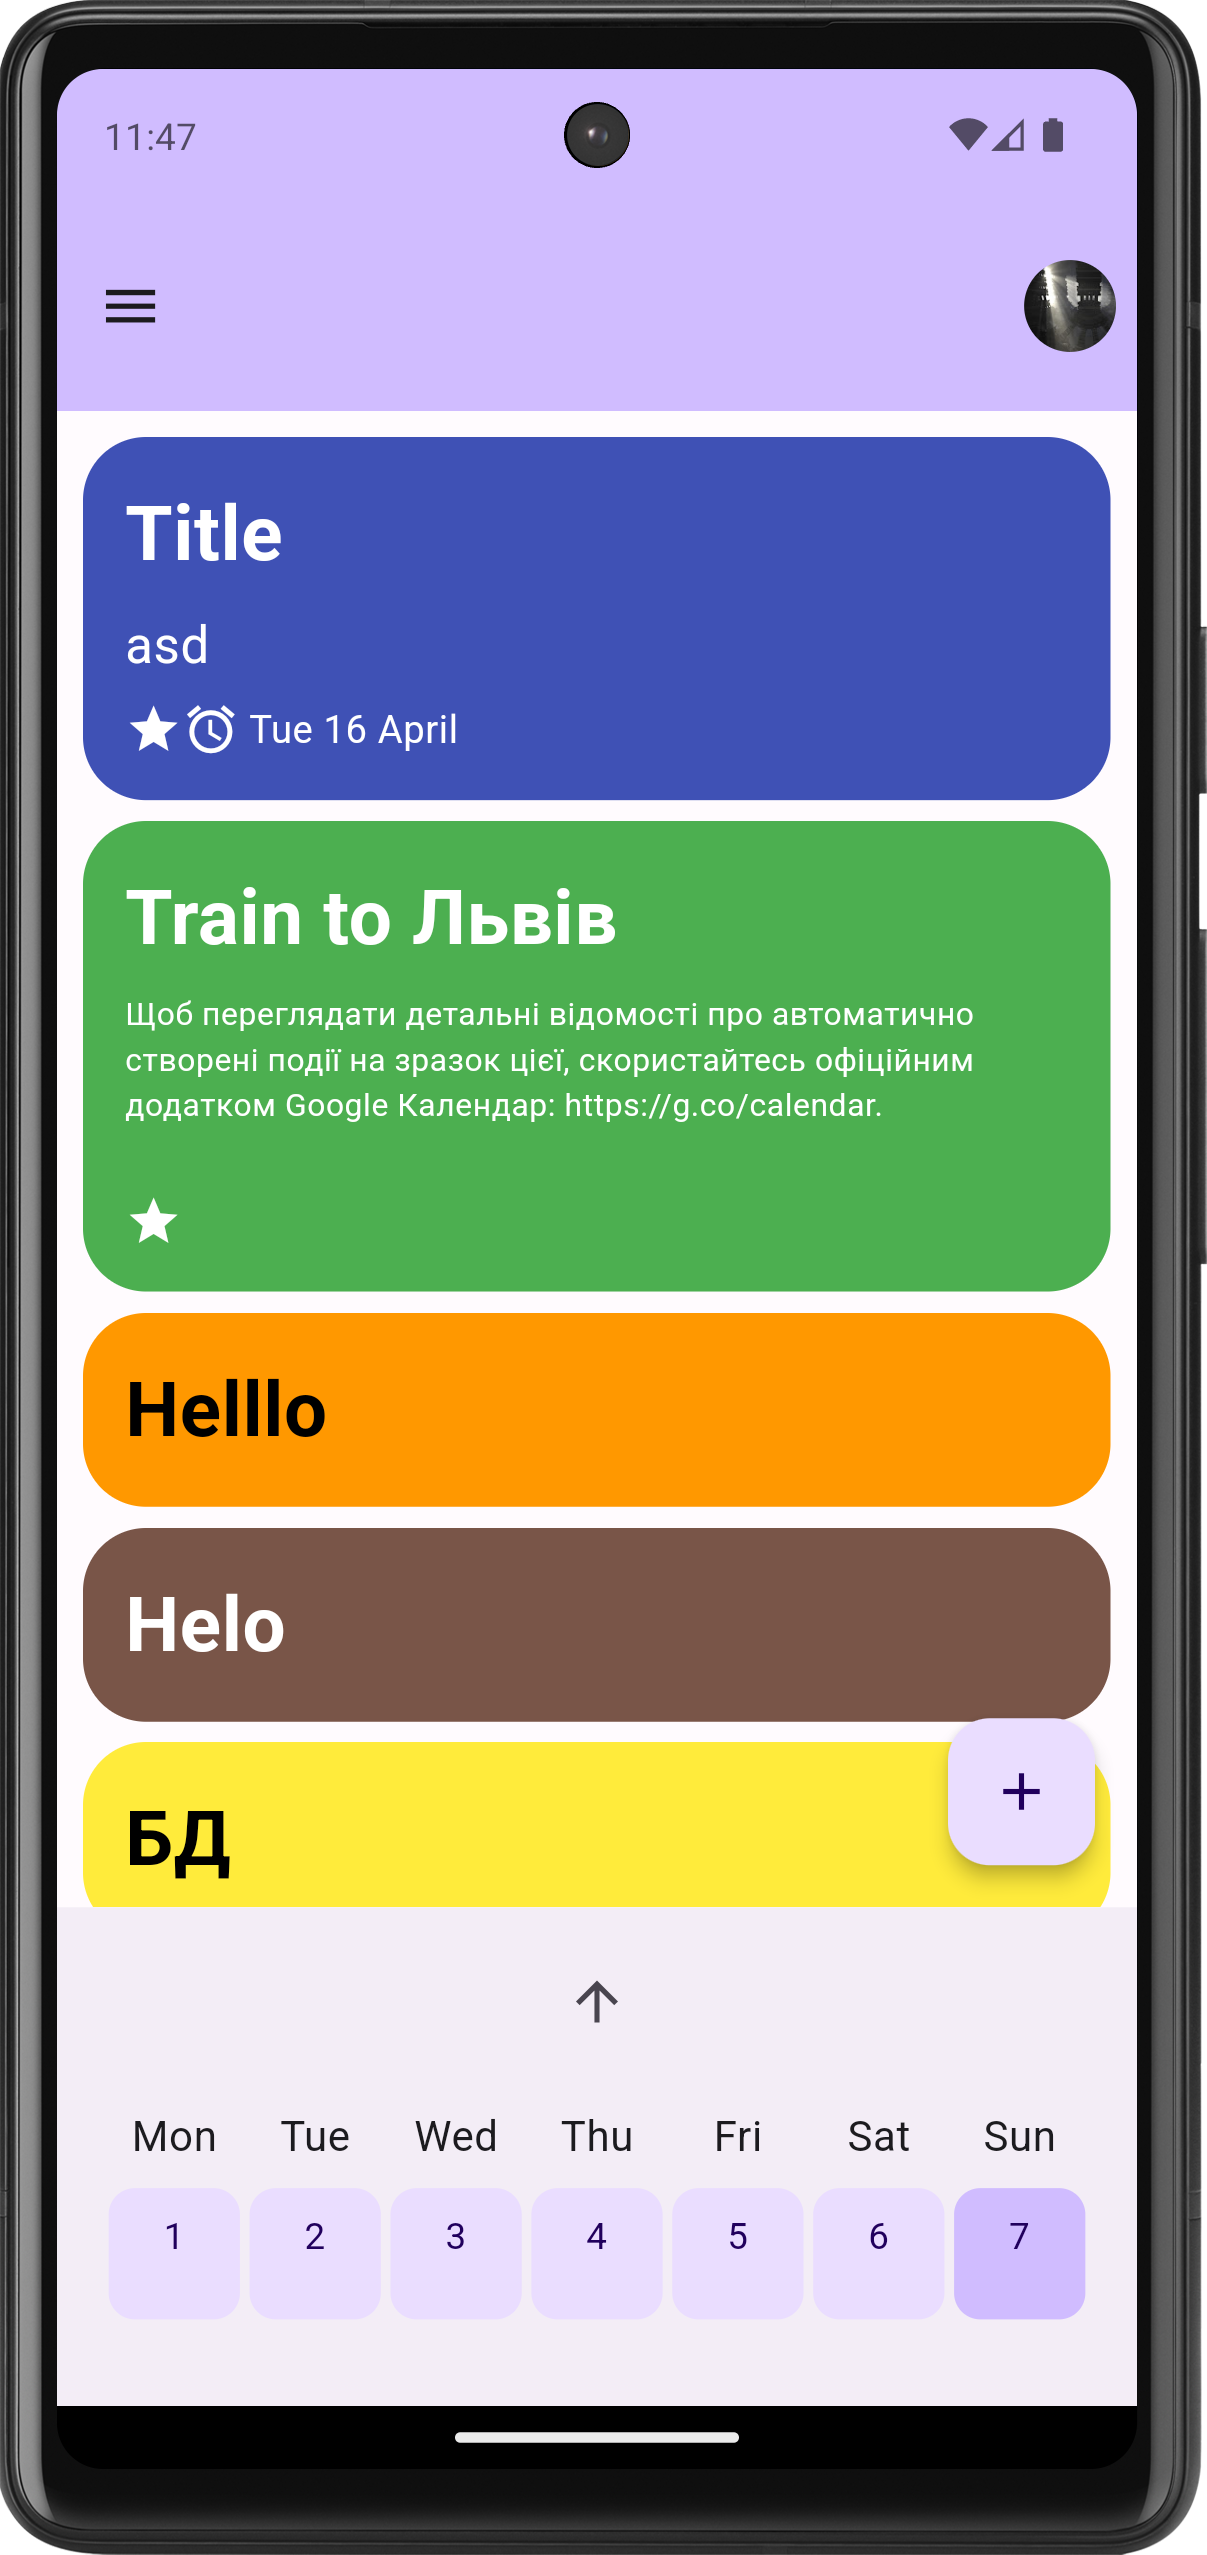
\includegraphics[scale=0.12]{1}
			\caption{Головний екран}
		\end{minipage}\hfill
		\begin{minipage}{0.48\textwidth}
			\centering
			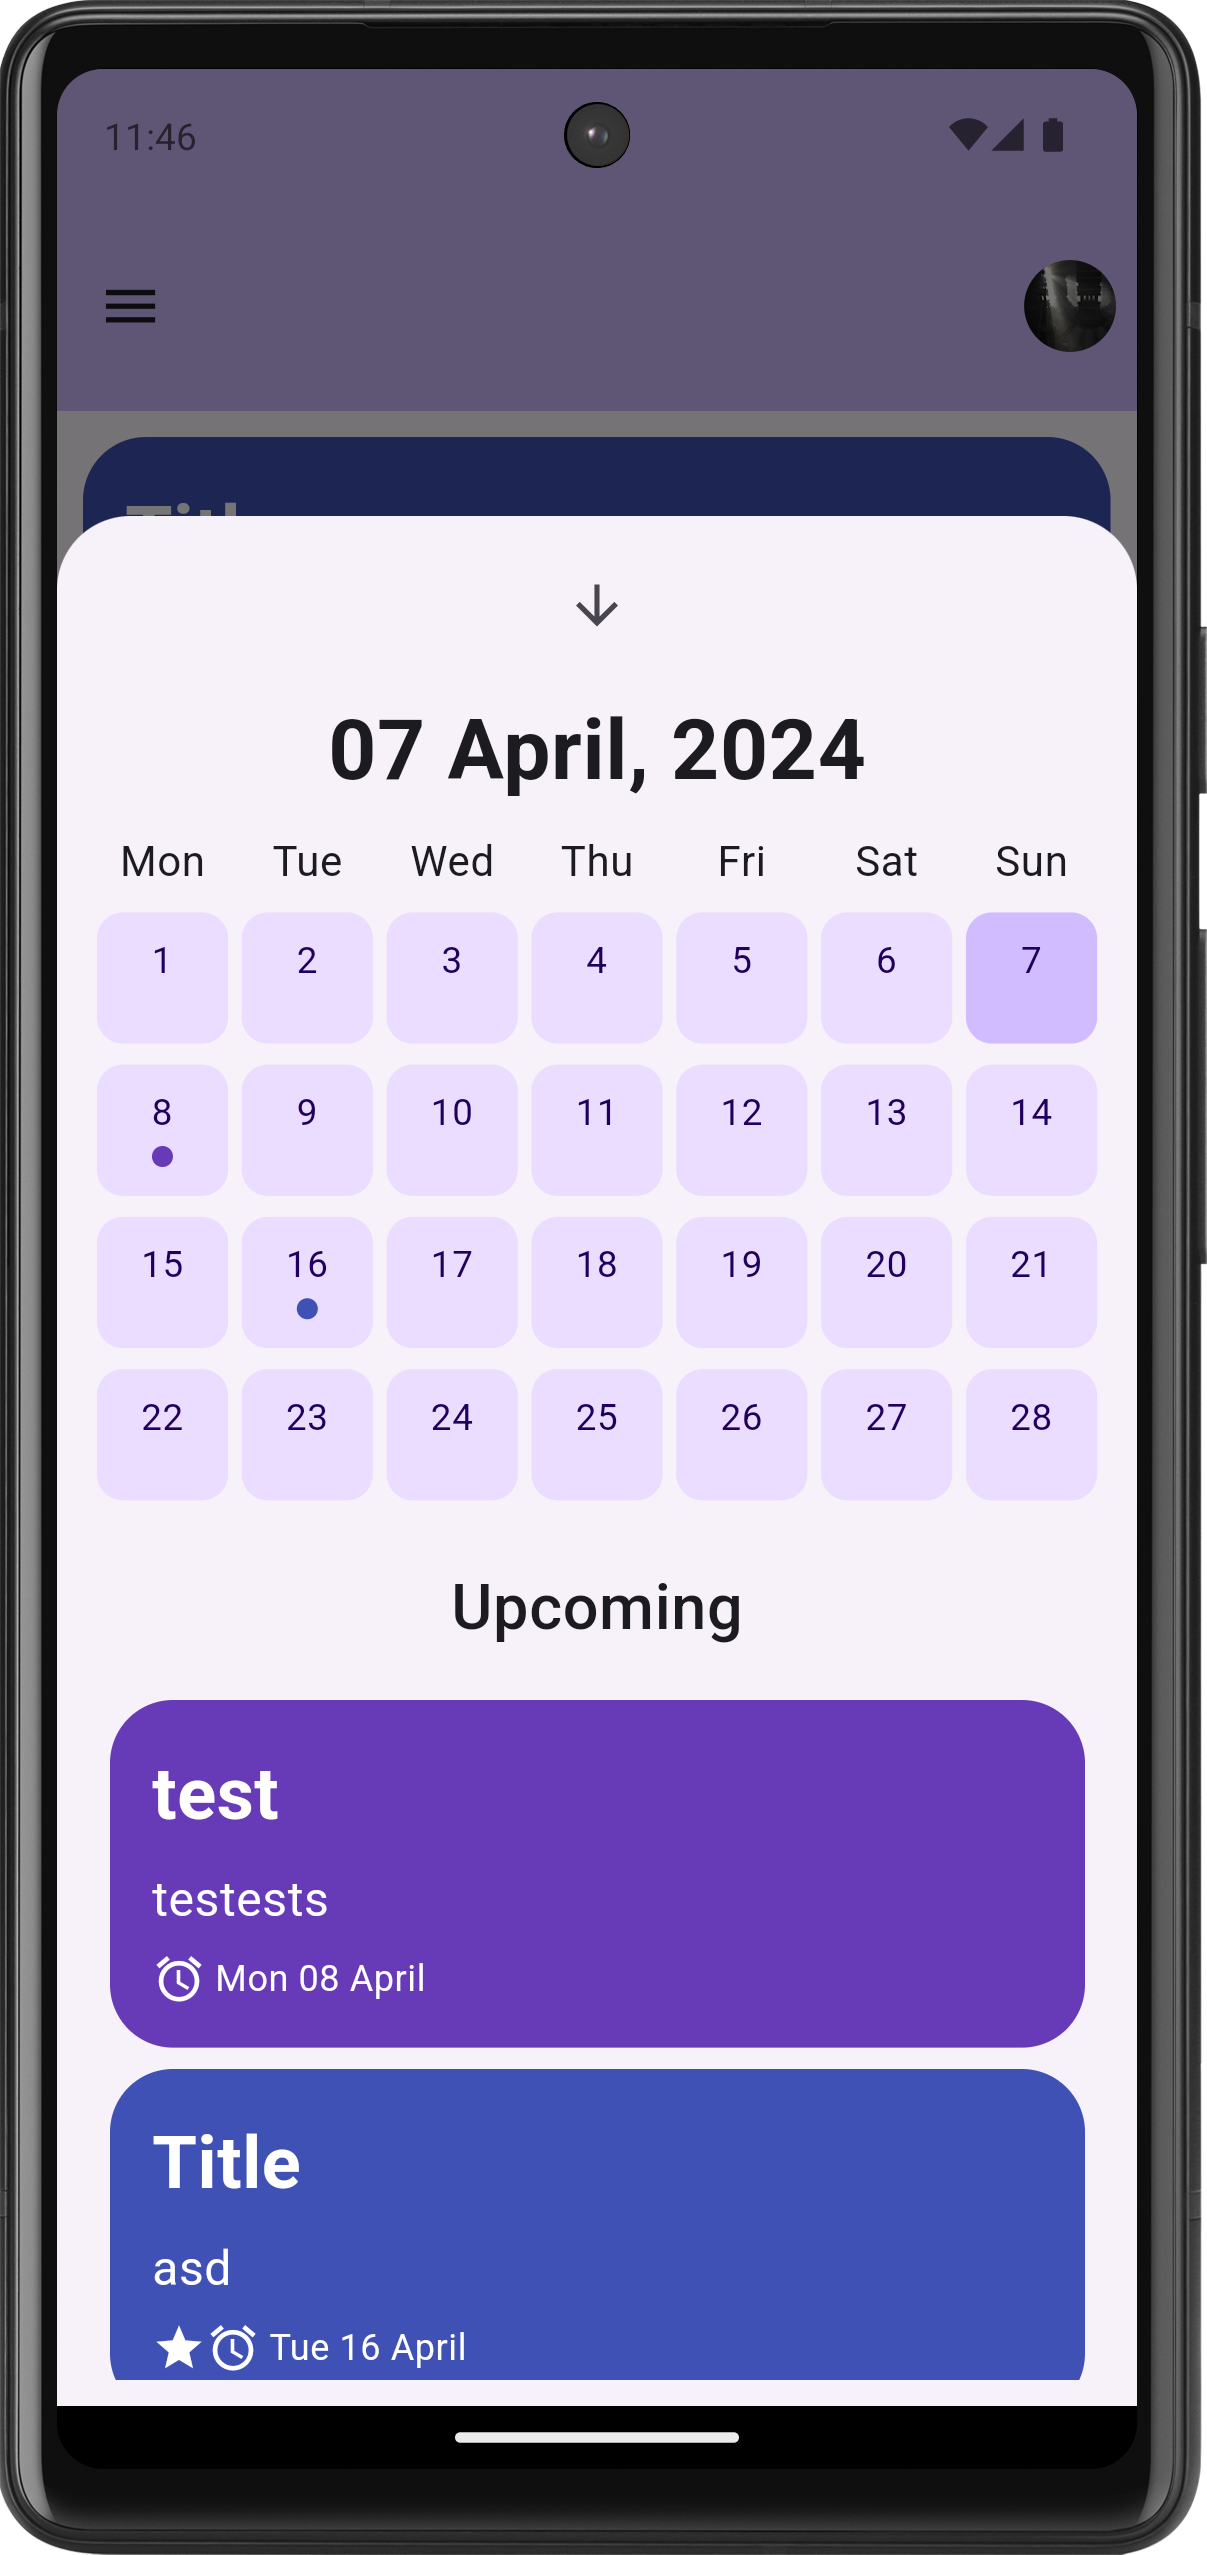
\includegraphics[scale=0.12]{2}
			\caption{Вікно з календарем та найближчими подіями}
		\end{minipage}
	\end{figure}
	
	\begin{figure}[H]
		\begin{minipage}{0.48\textwidth}
			\centering
			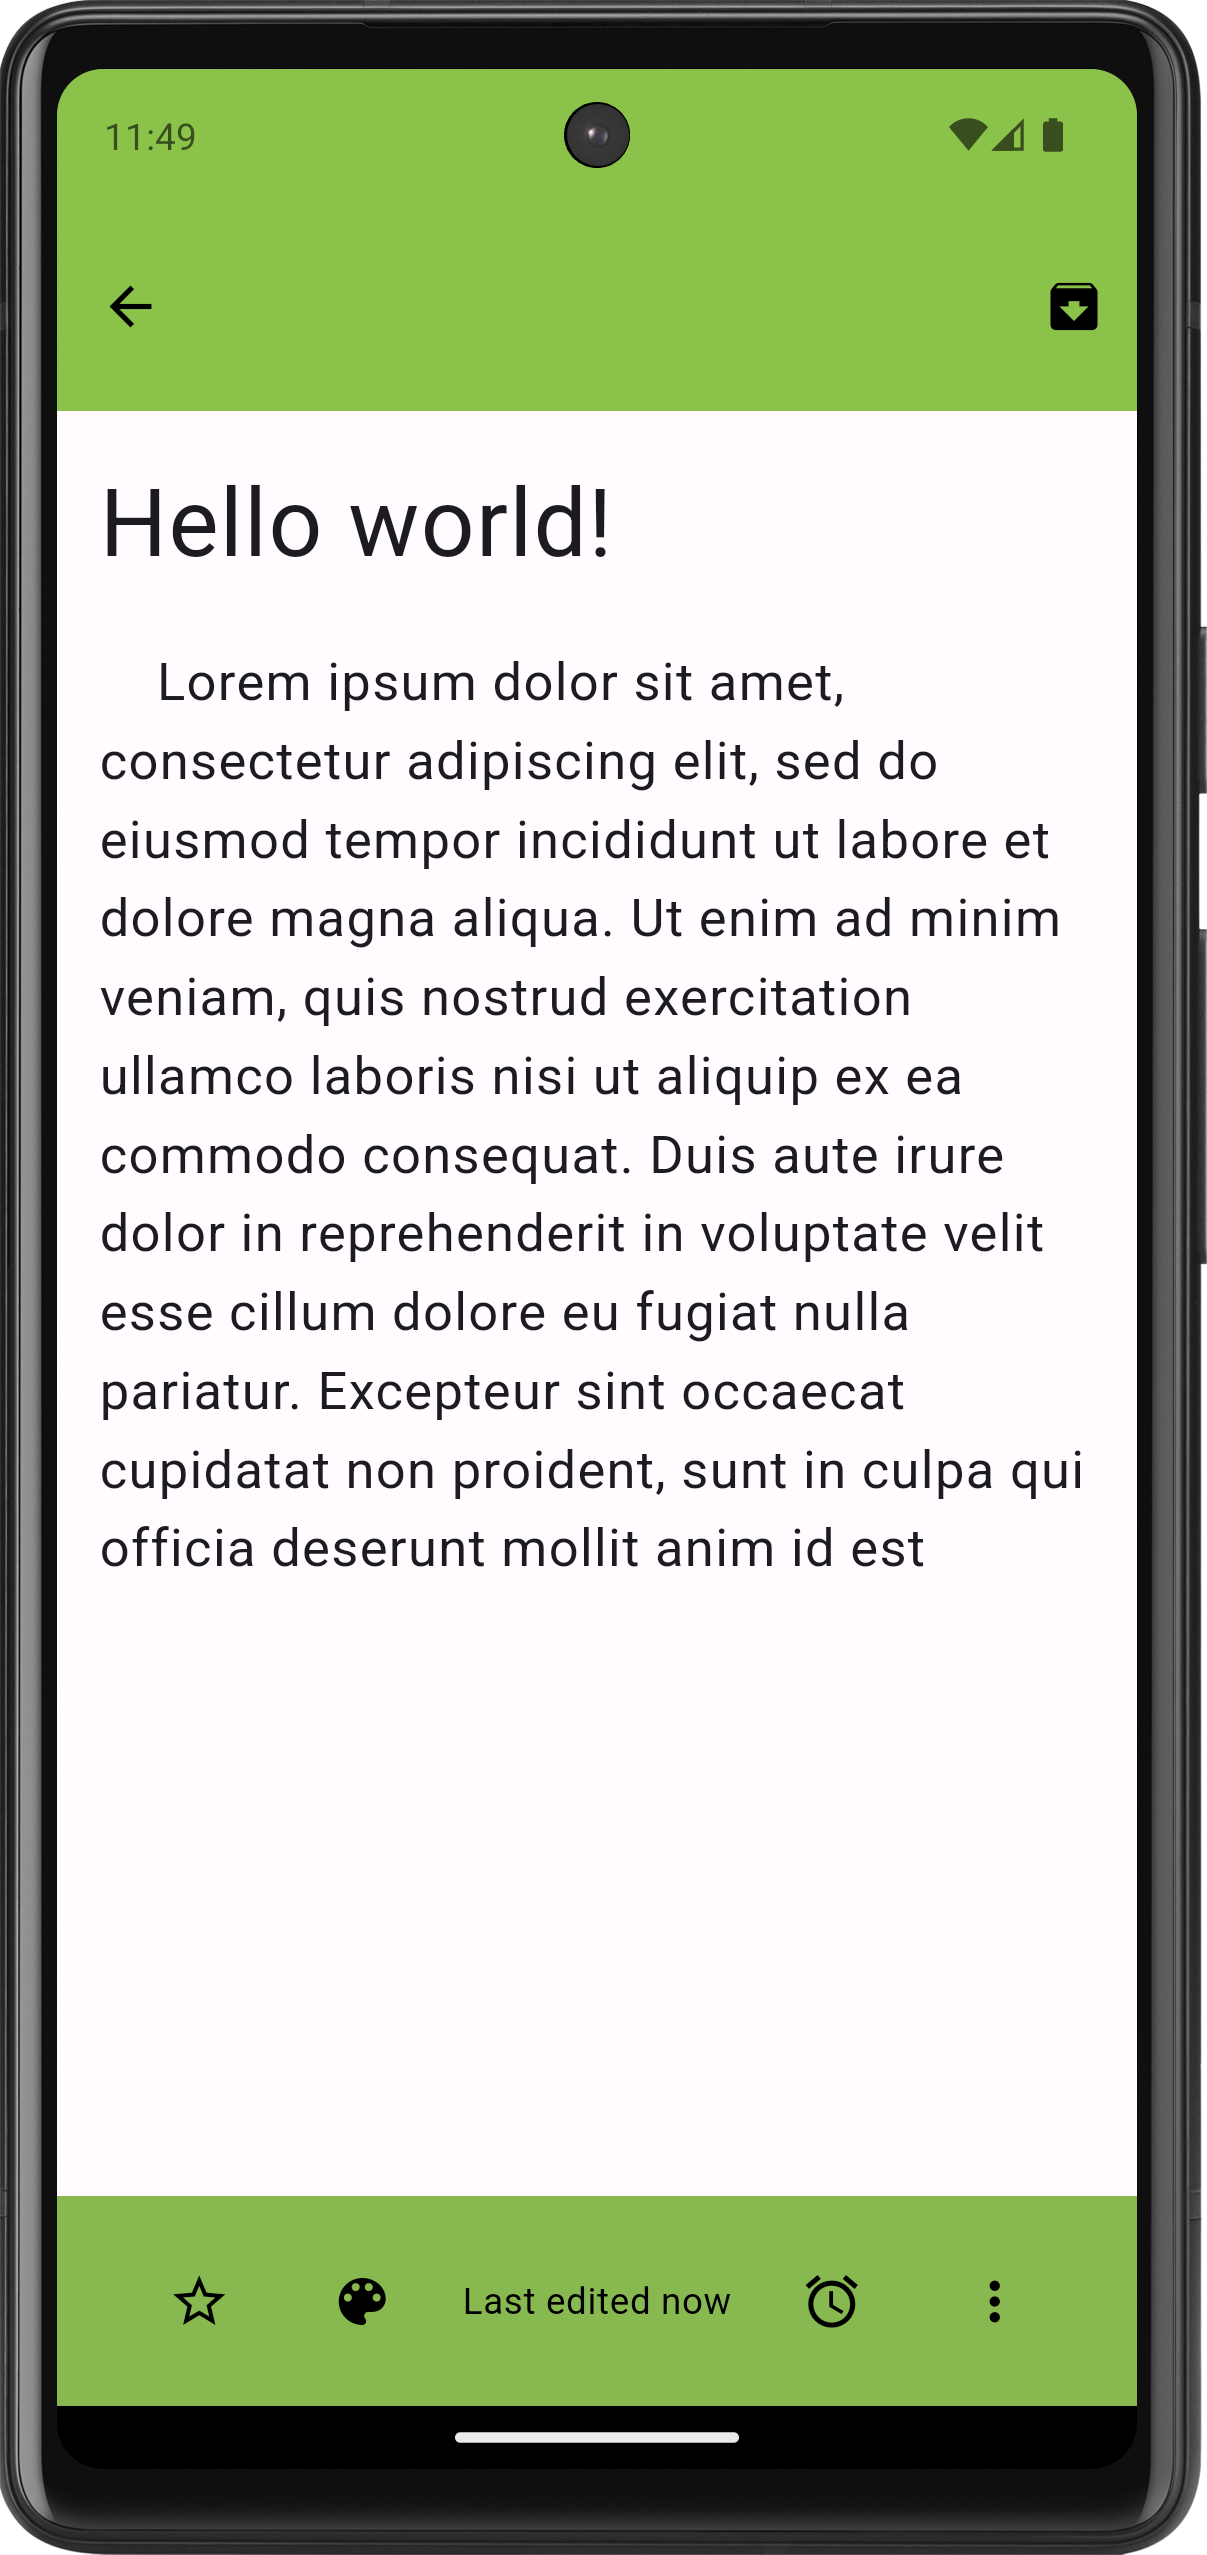
\includegraphics[scale=0.12]{3}
			\caption{Редагування нотатки}
		\end{minipage}\hfill
		\begin{minipage}{0.48\textwidth}
			\centering
			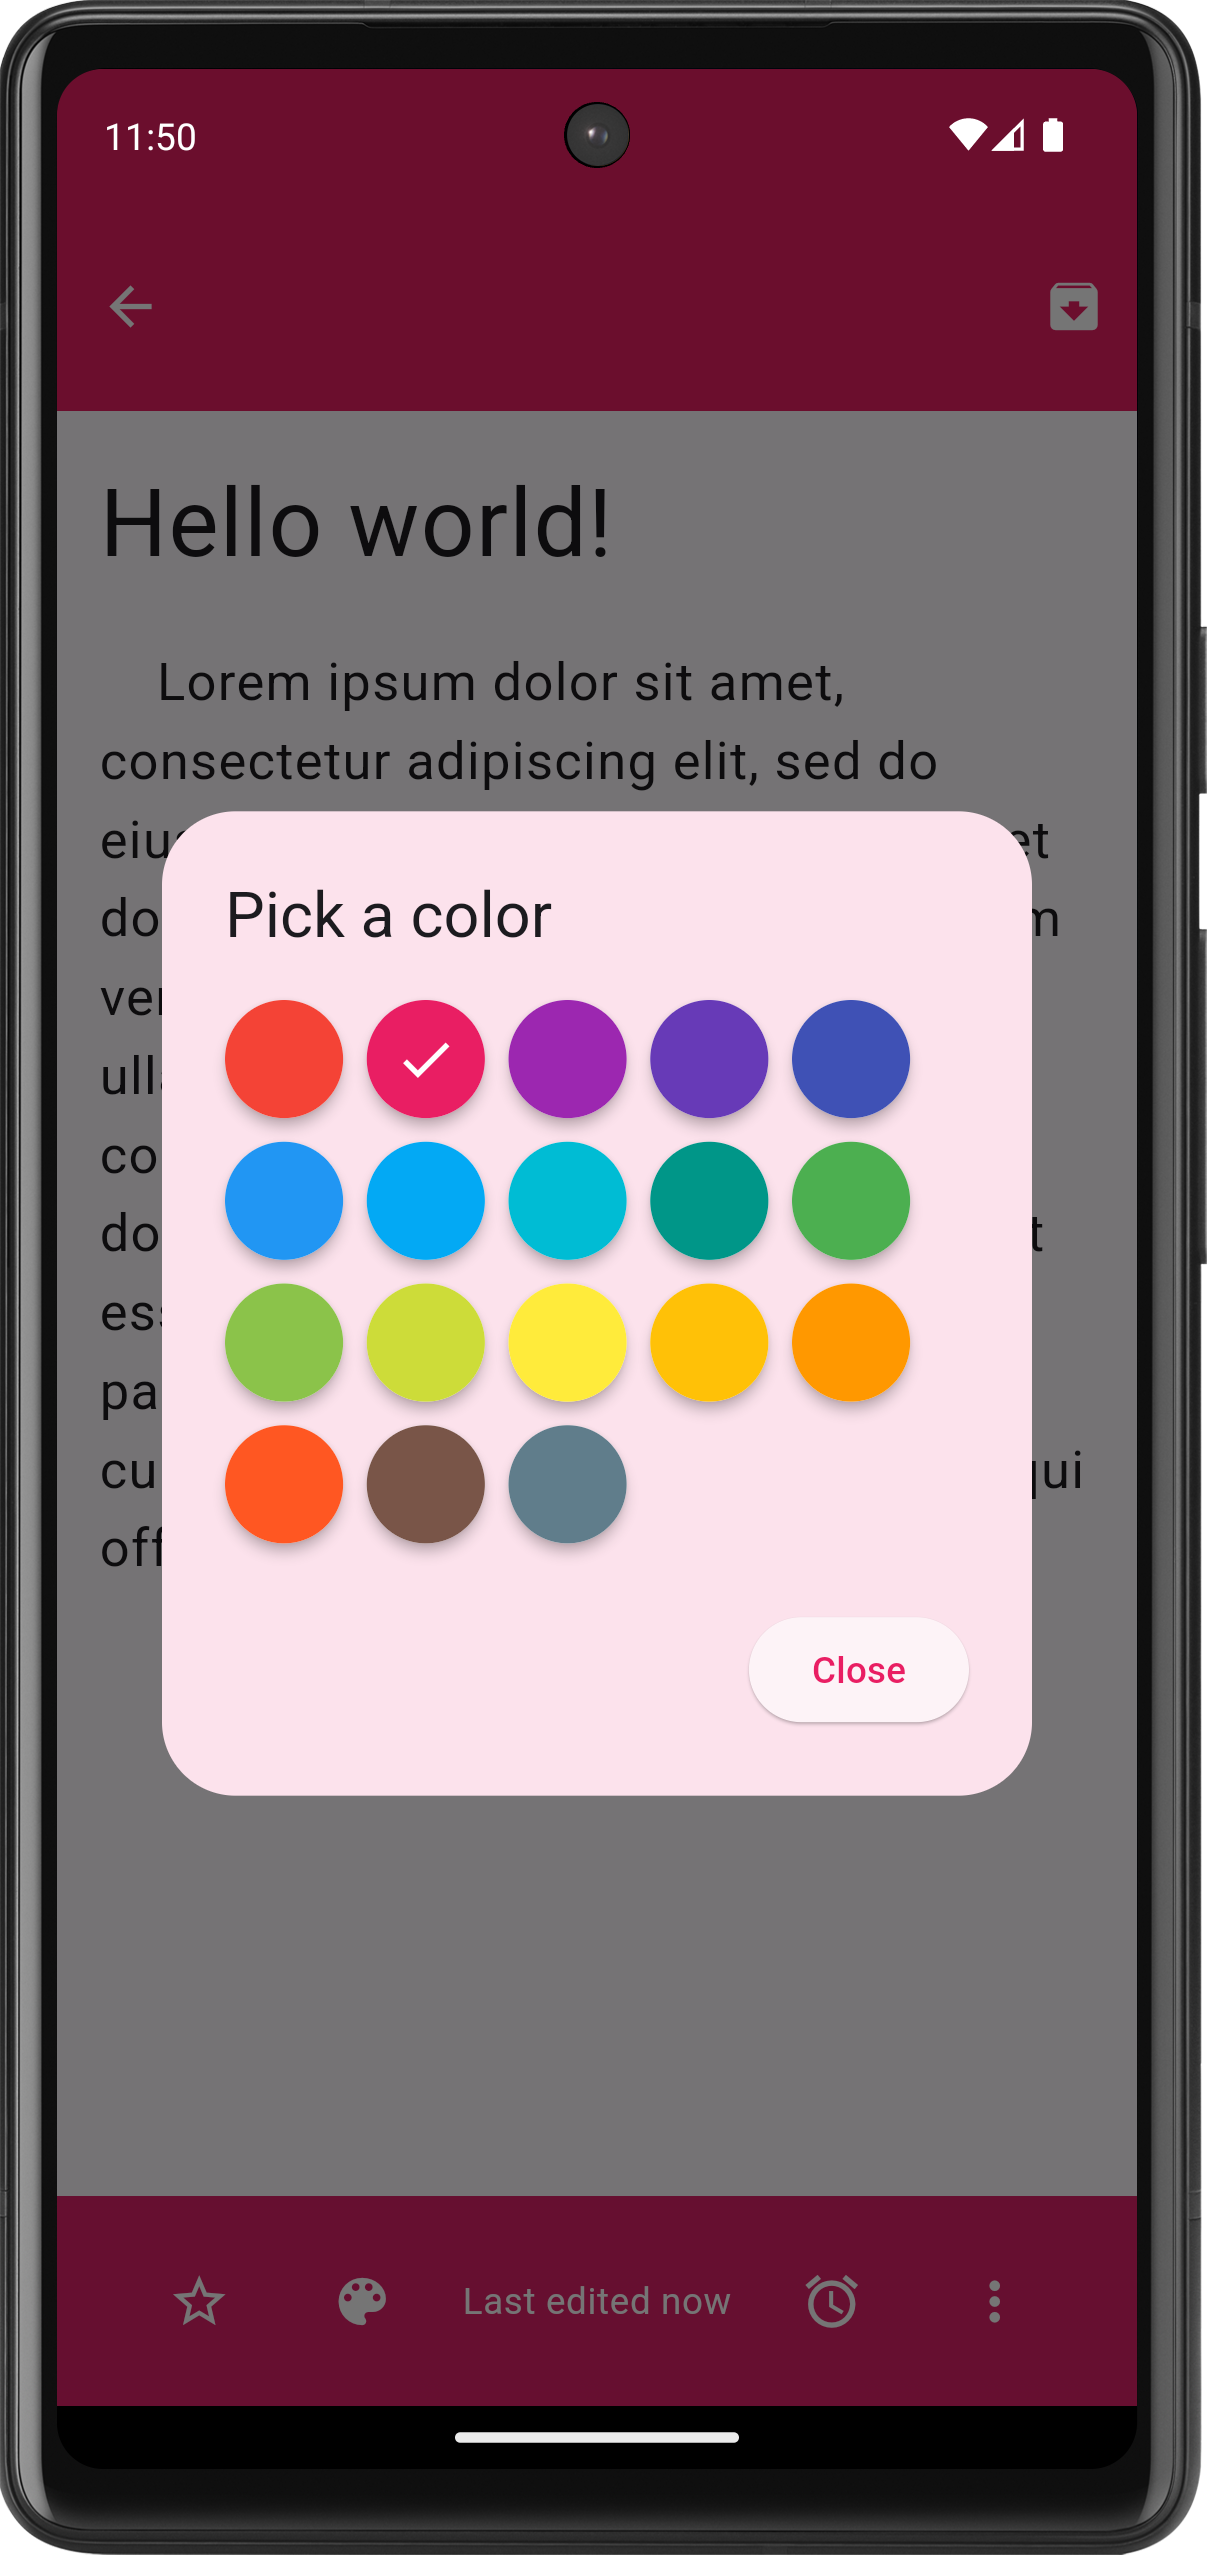
\includegraphics[scale=0.12]{4}
			\caption{Редагування нотатки: вибір акцентного кольору}
		\end{minipage}
	\end{figure}
	
	
	\begin{figure}[H]
		\begin{minipage}{0.48\textwidth}
			\centering
			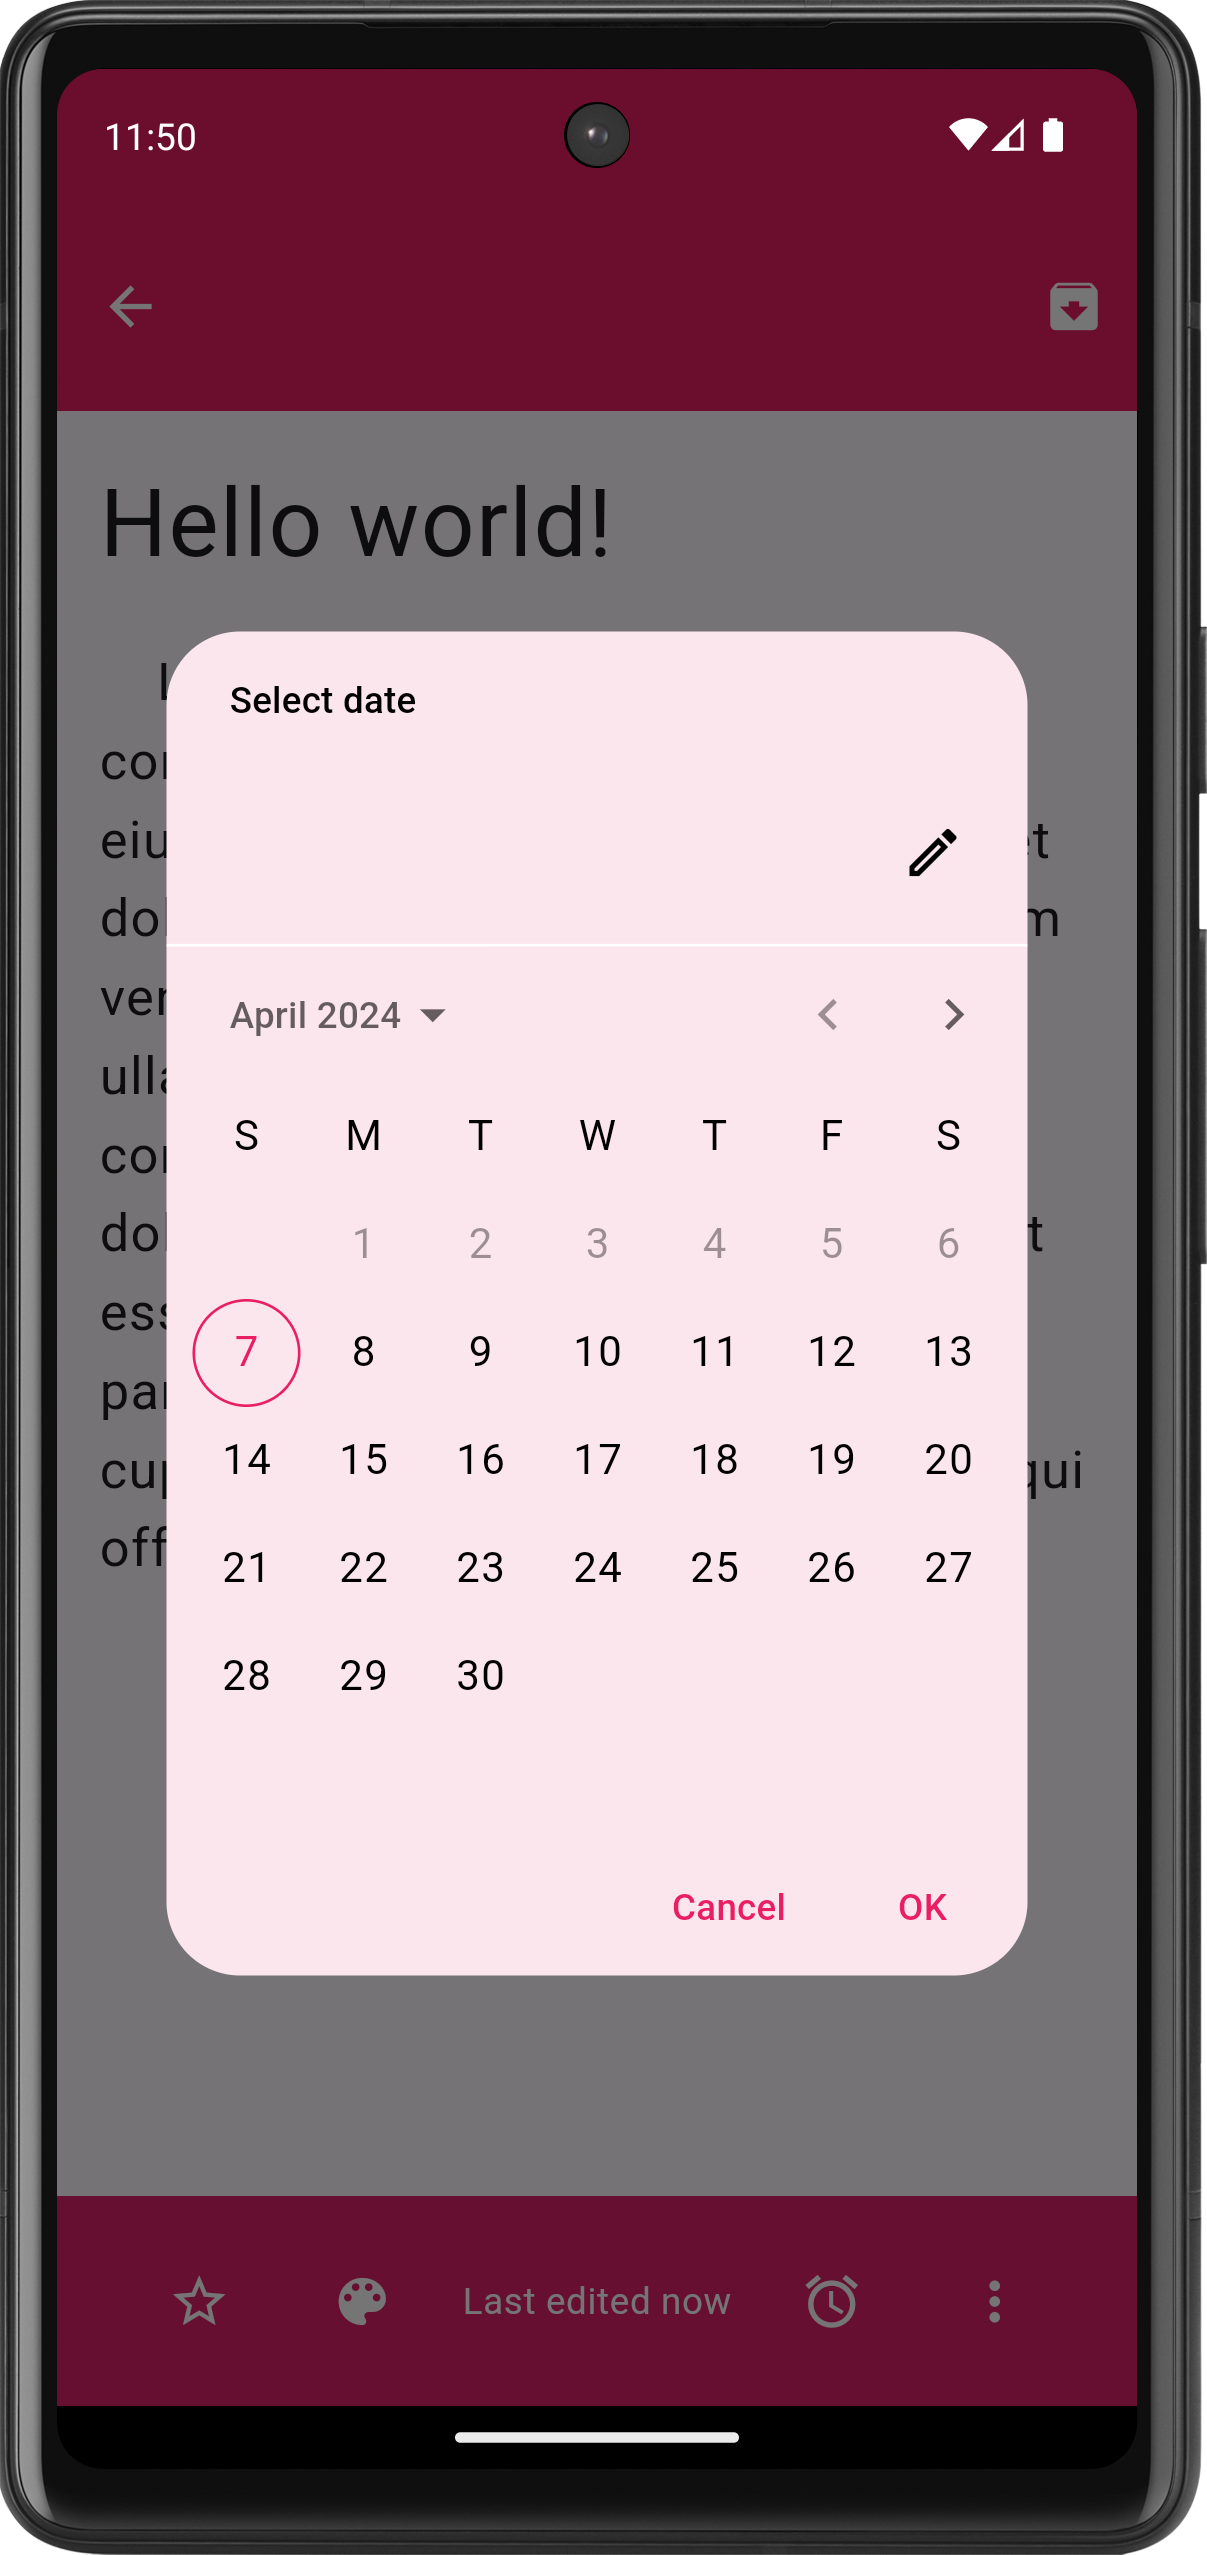
\includegraphics[scale=0.12]{5}
			\caption{Редагування нотатки: вибір часу для нагадування}
		\end{minipage}\hfill
		\begin{minipage}{0.48\textwidth}
			\centering
			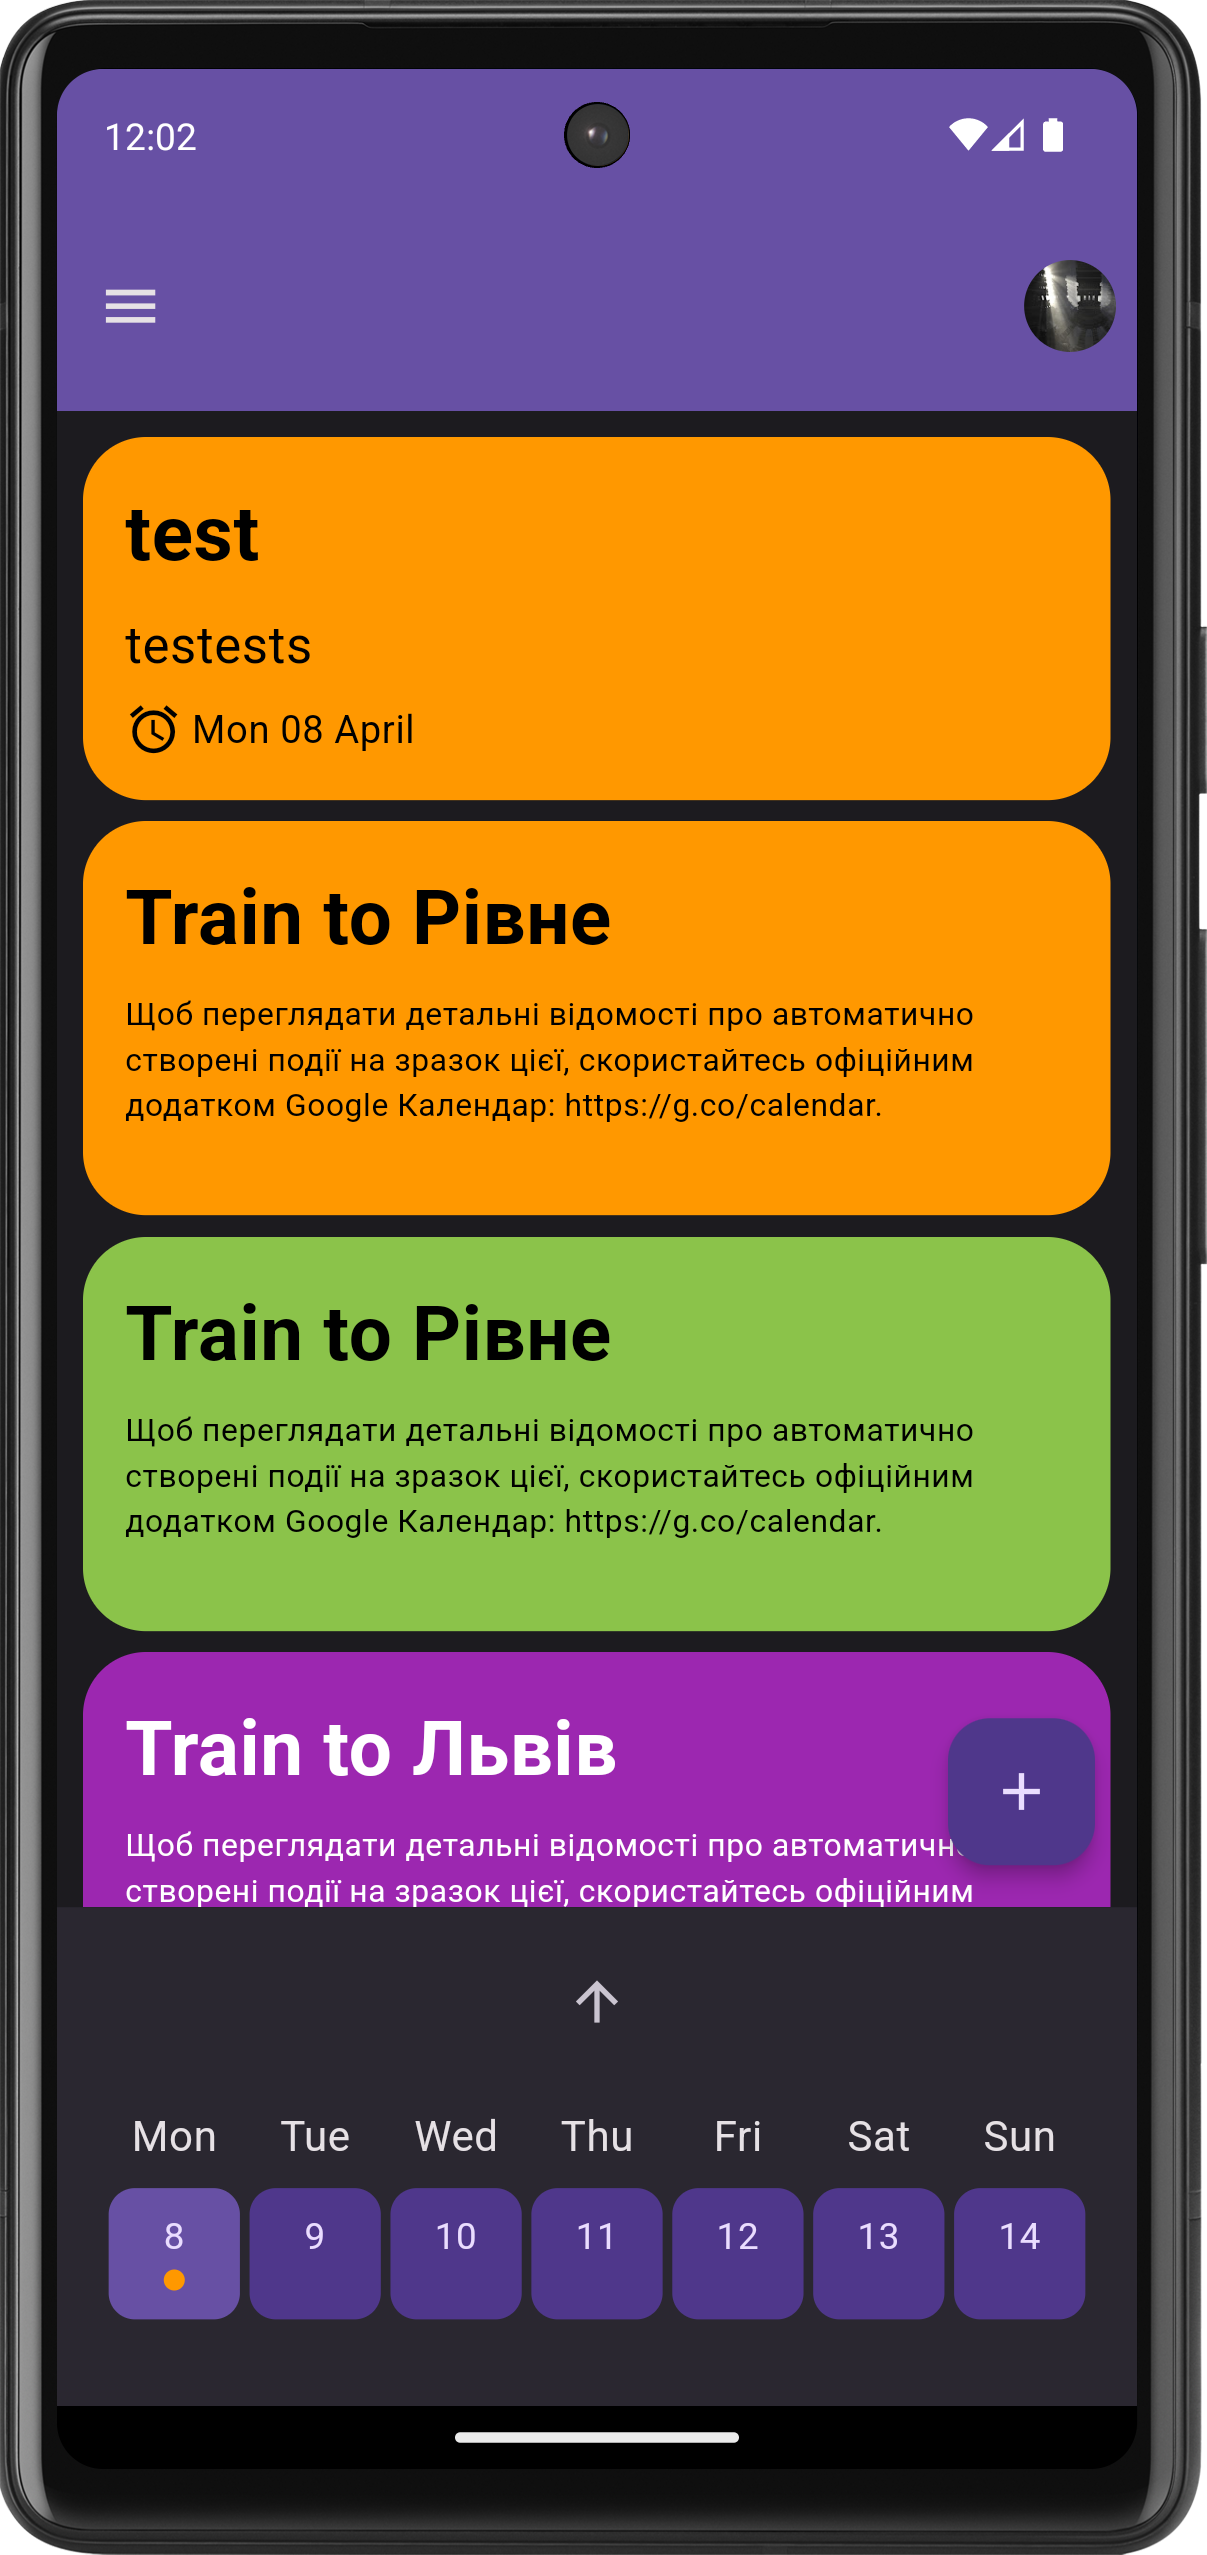
\includegraphics[scale=0.12]{9}
			\caption{Підтримка темної теми}
		\end{minipage}
	\end{figure}
	
	\begin{figure}[H]
		\begin{minipage}{0.48\textwidth}
			\centering
			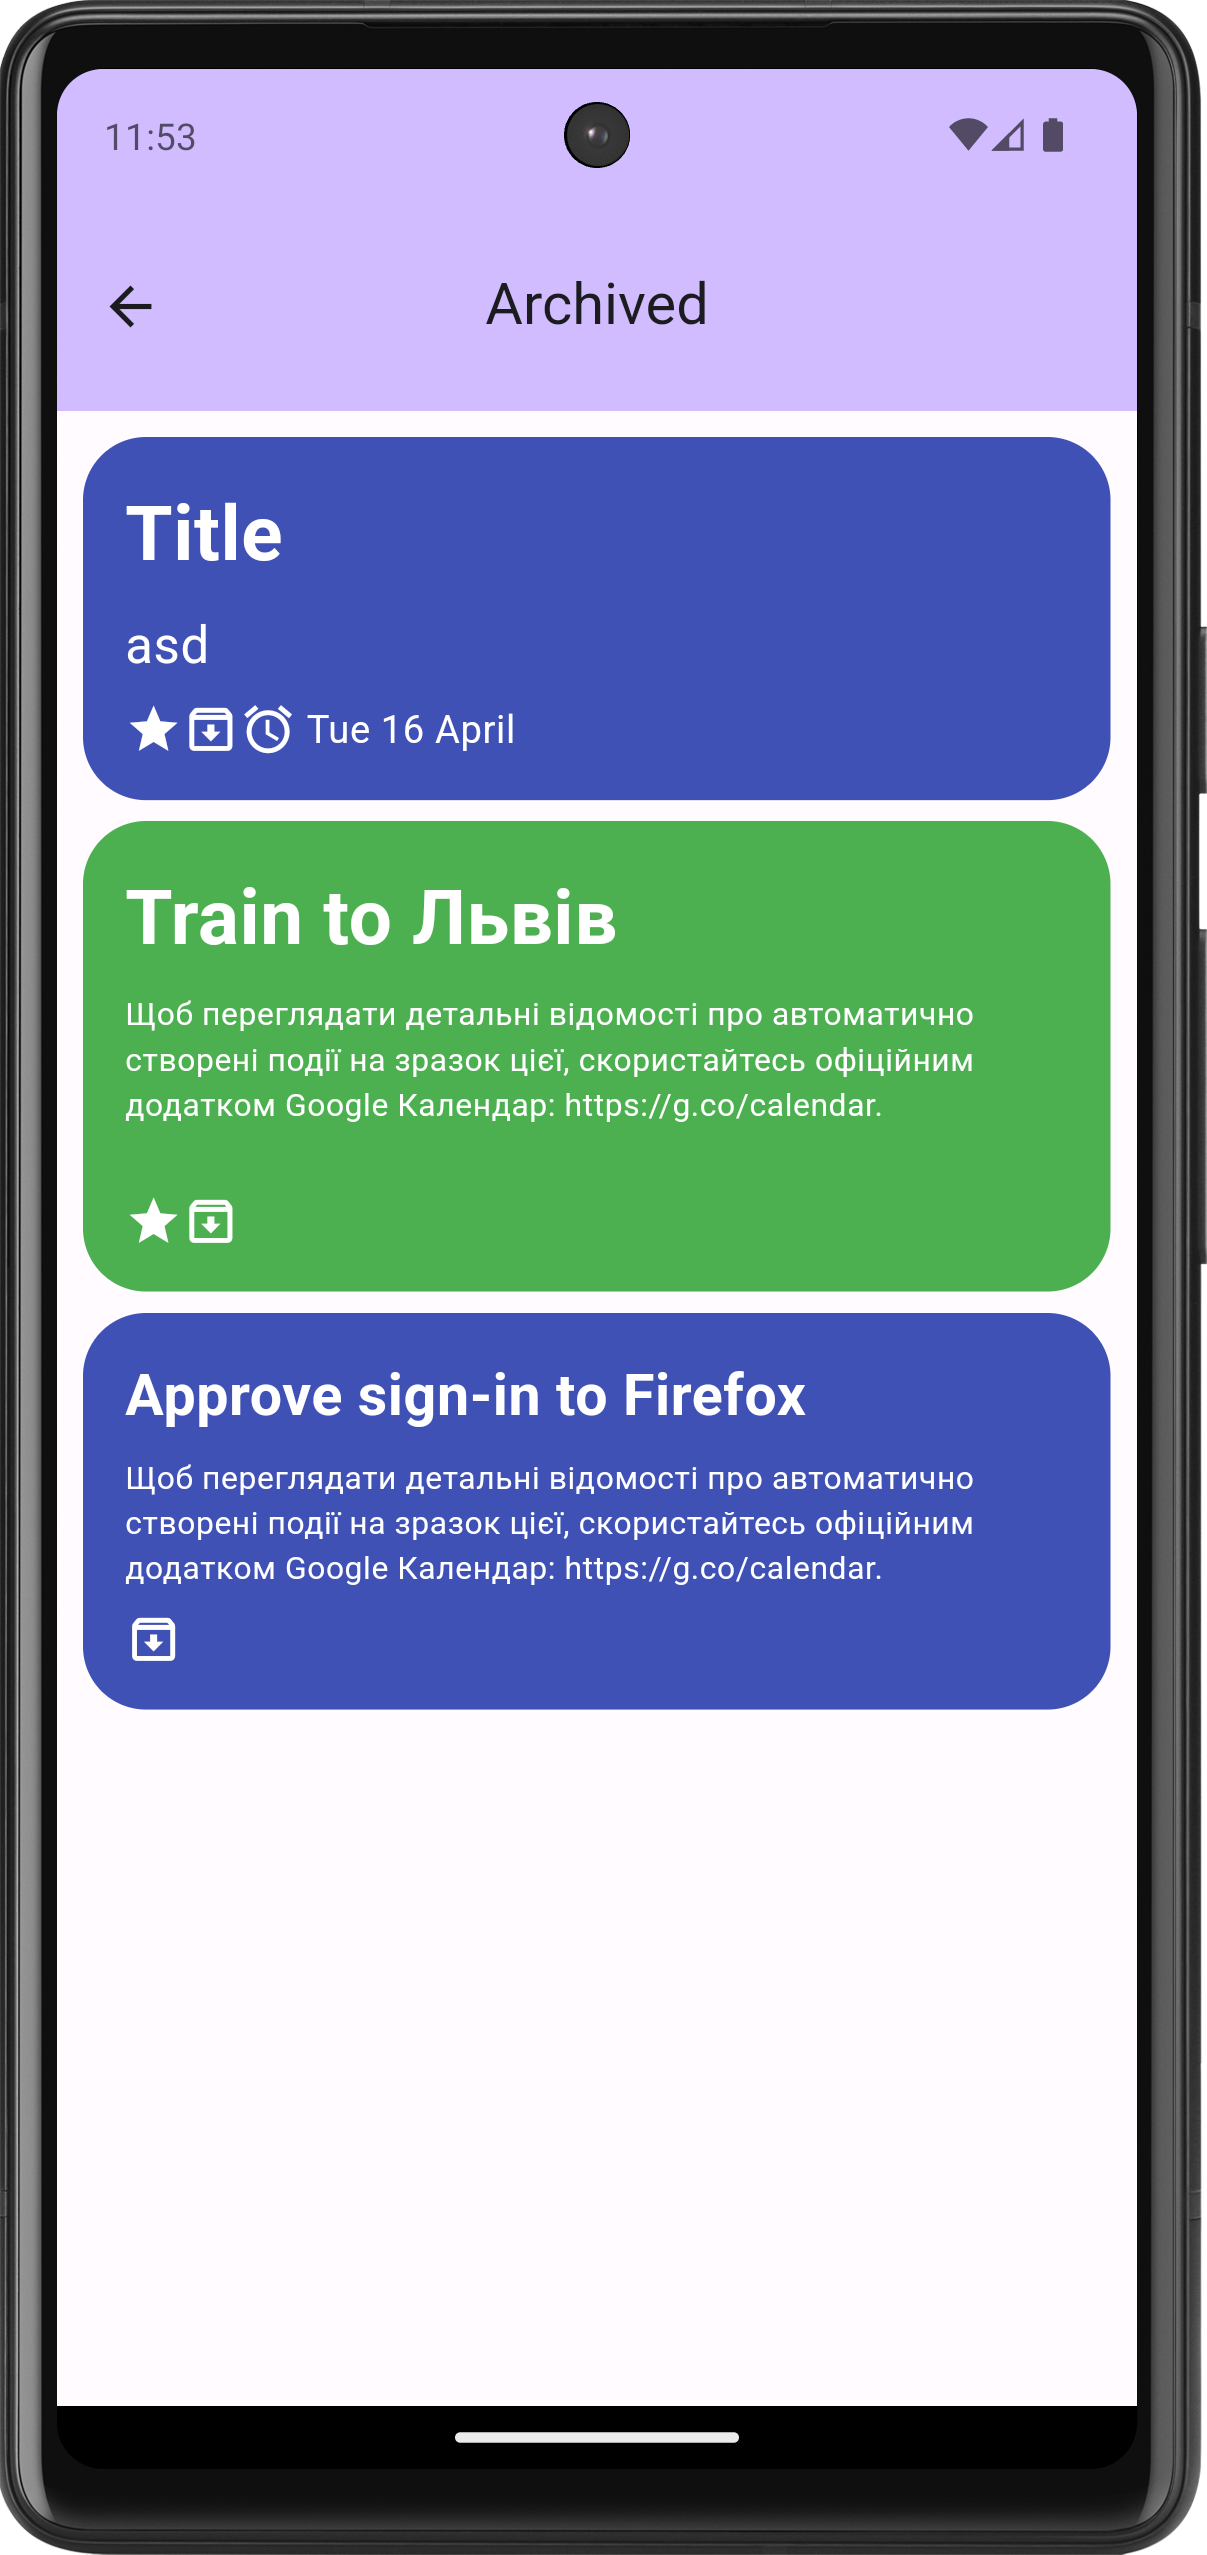
\includegraphics[scale=0.12]{7}
			\caption{Список архівованих нотаток}
		\end{minipage}\hfill
		\begin{minipage}{0.48\textwidth}
			\centering
			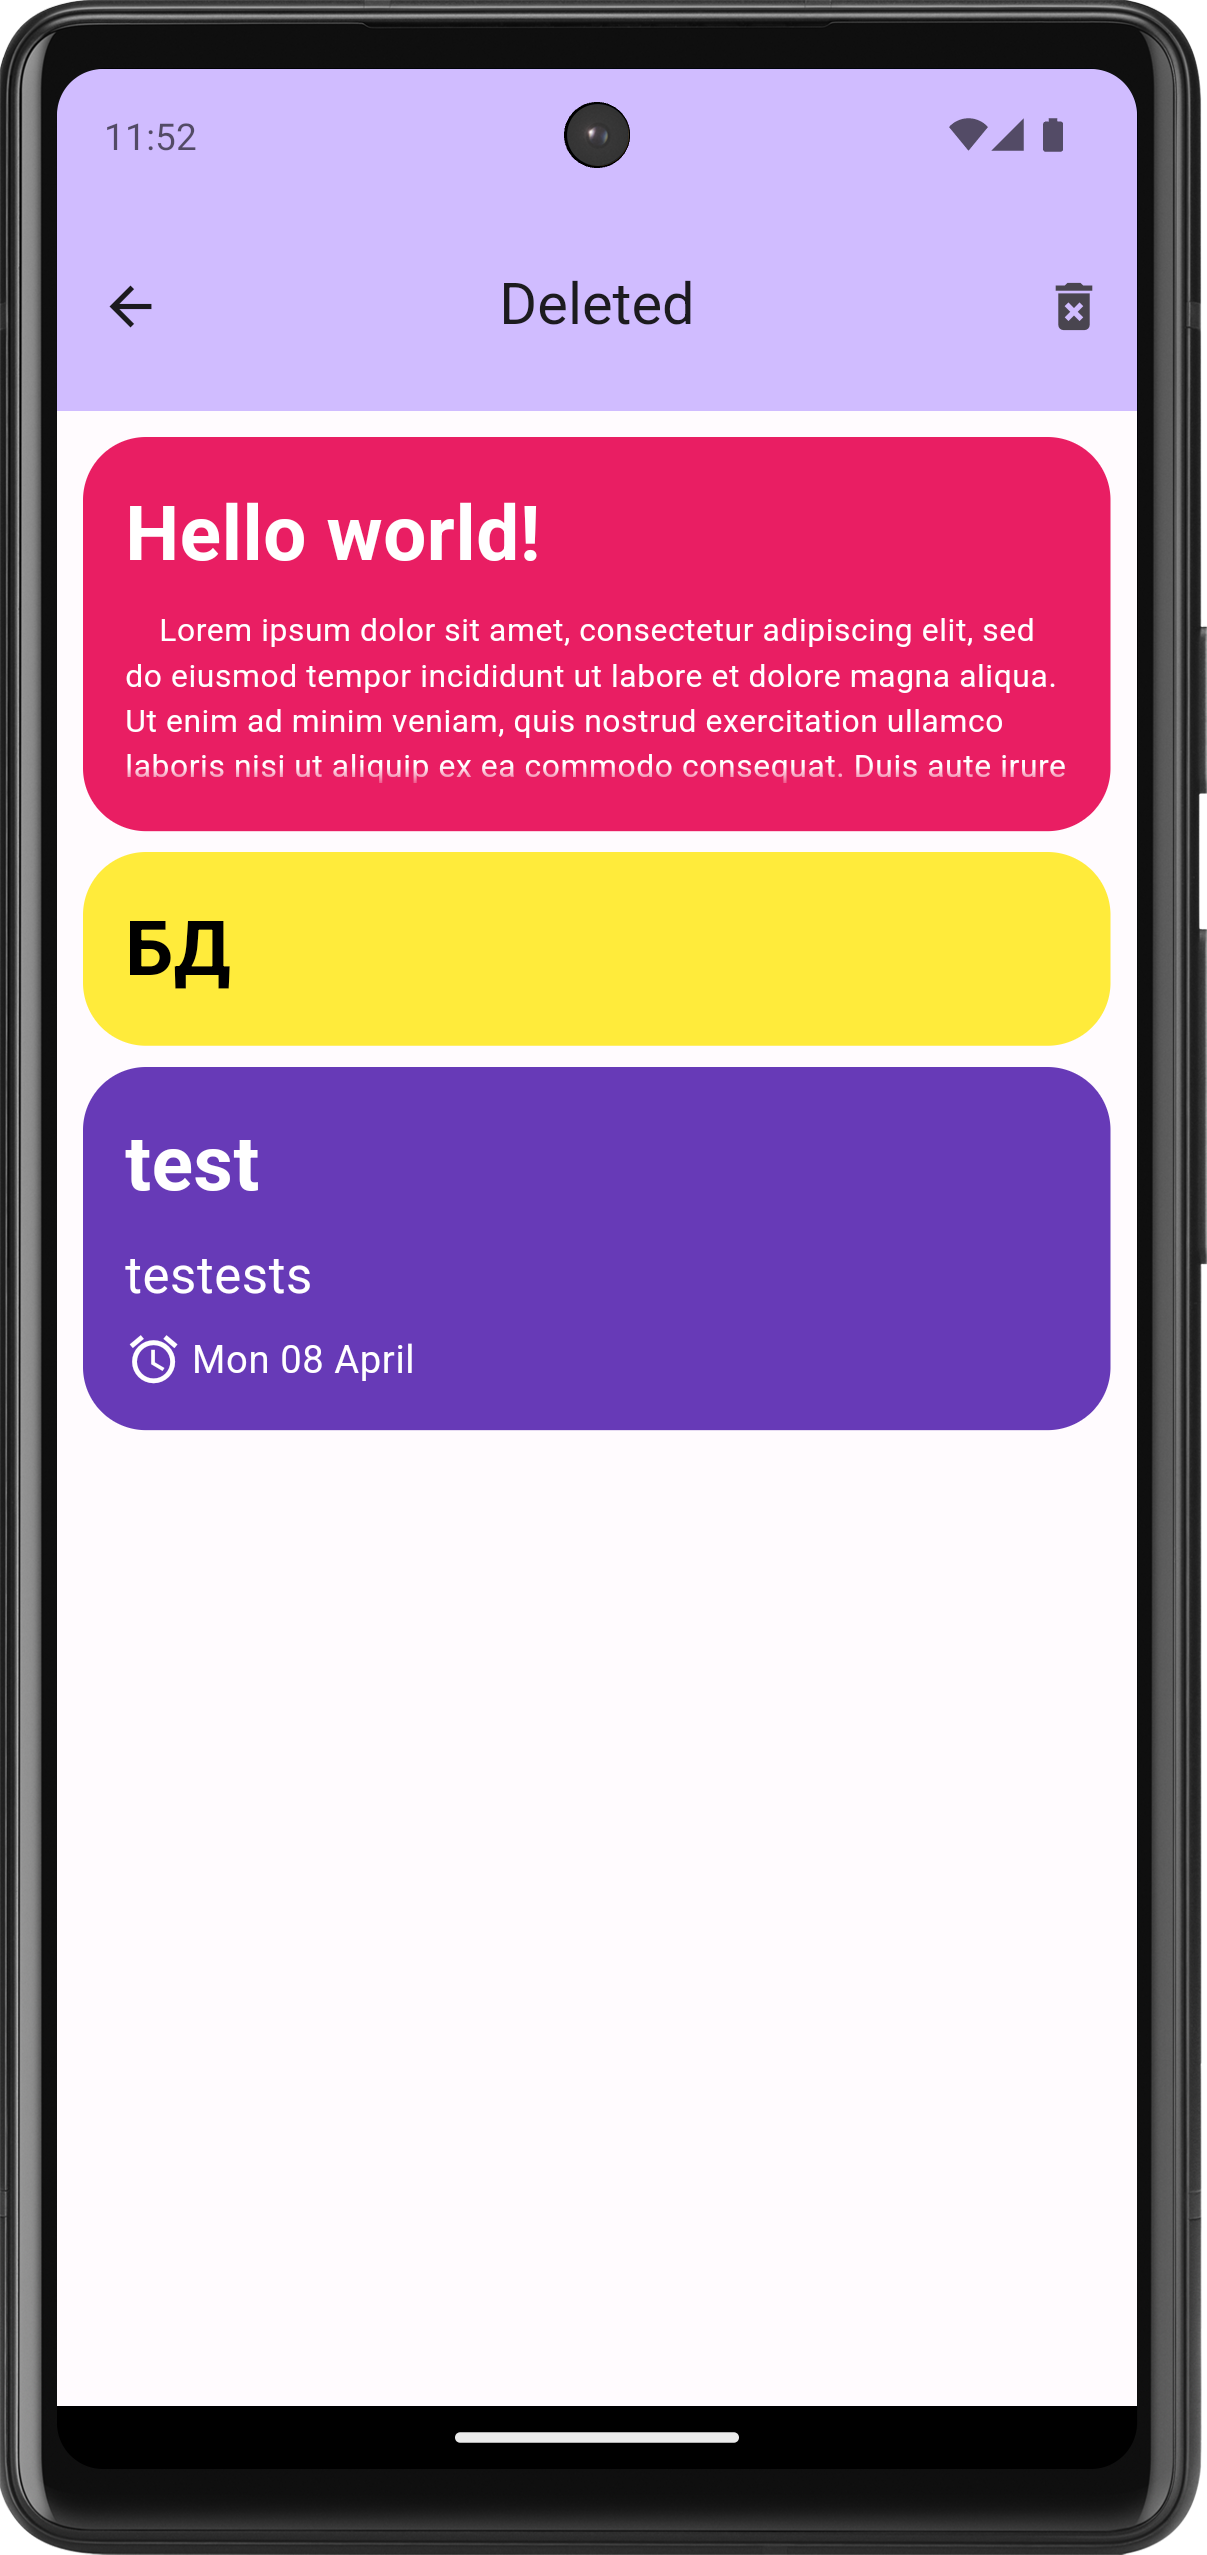
\includegraphics[scale=0.12]{6}
			\caption{Список видалених нотаток}
		\end{minipage}
	\end{figure}
	
	\begin{figure}[H]
		\begin{minipage}{0.48\textwidth}
			\centering
			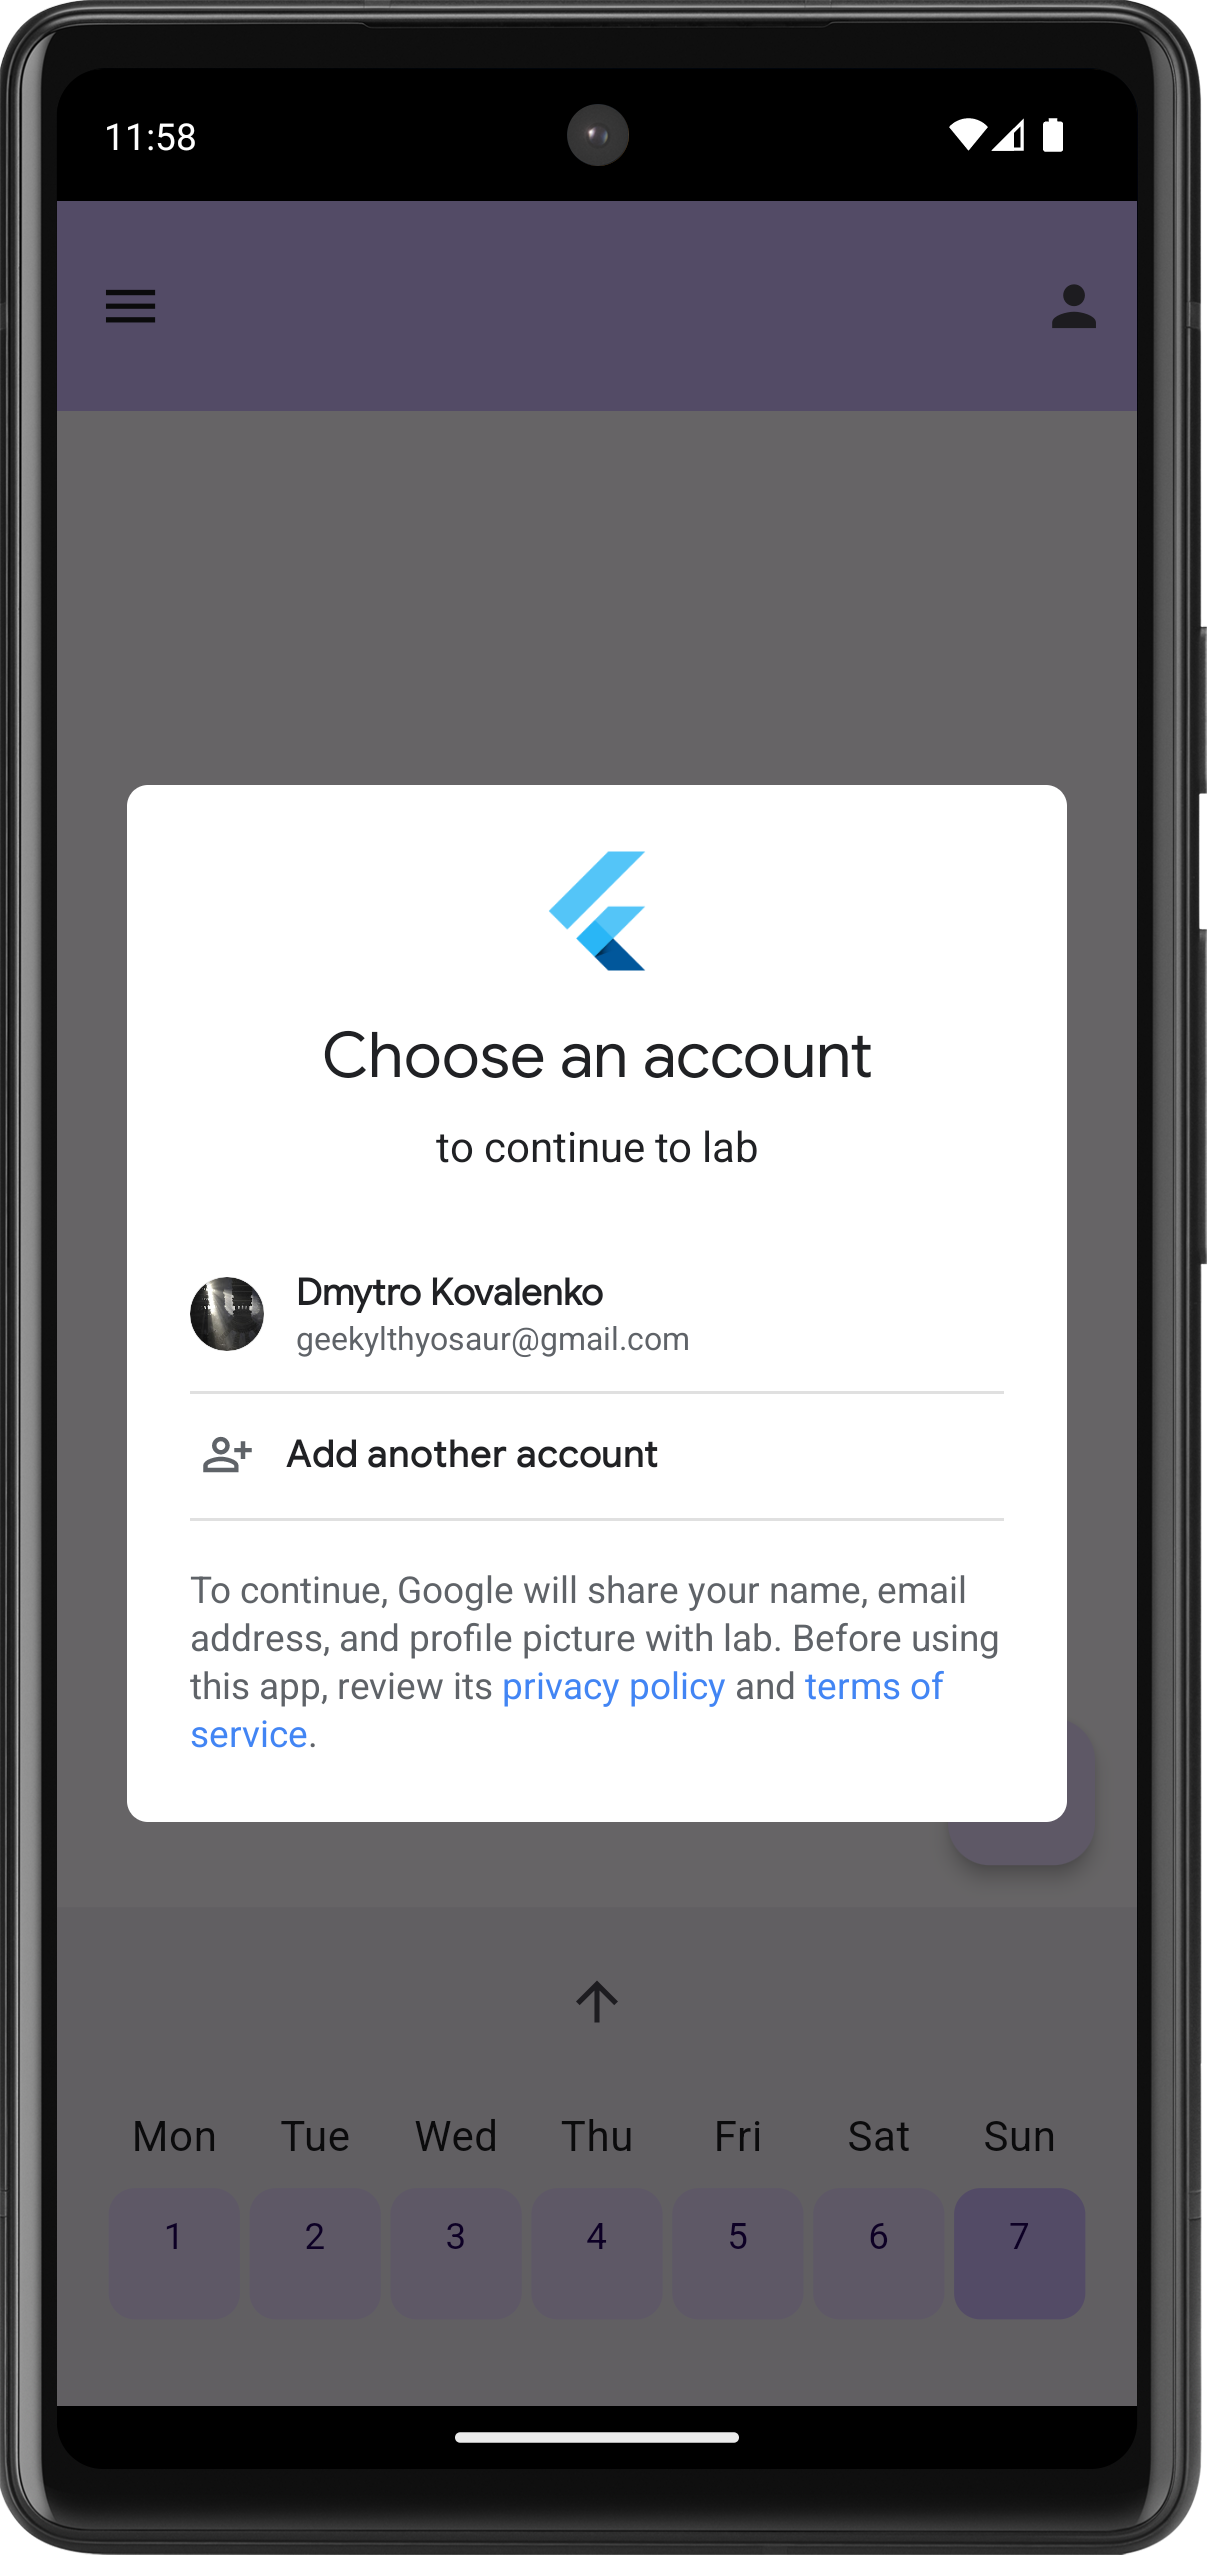
\includegraphics[scale=0.12]{10}
			\caption{Можливість входу в Google акаунт}
		\end{minipage}\hfill
		\begin{minipage}{0.48\textwidth}
			\centering
			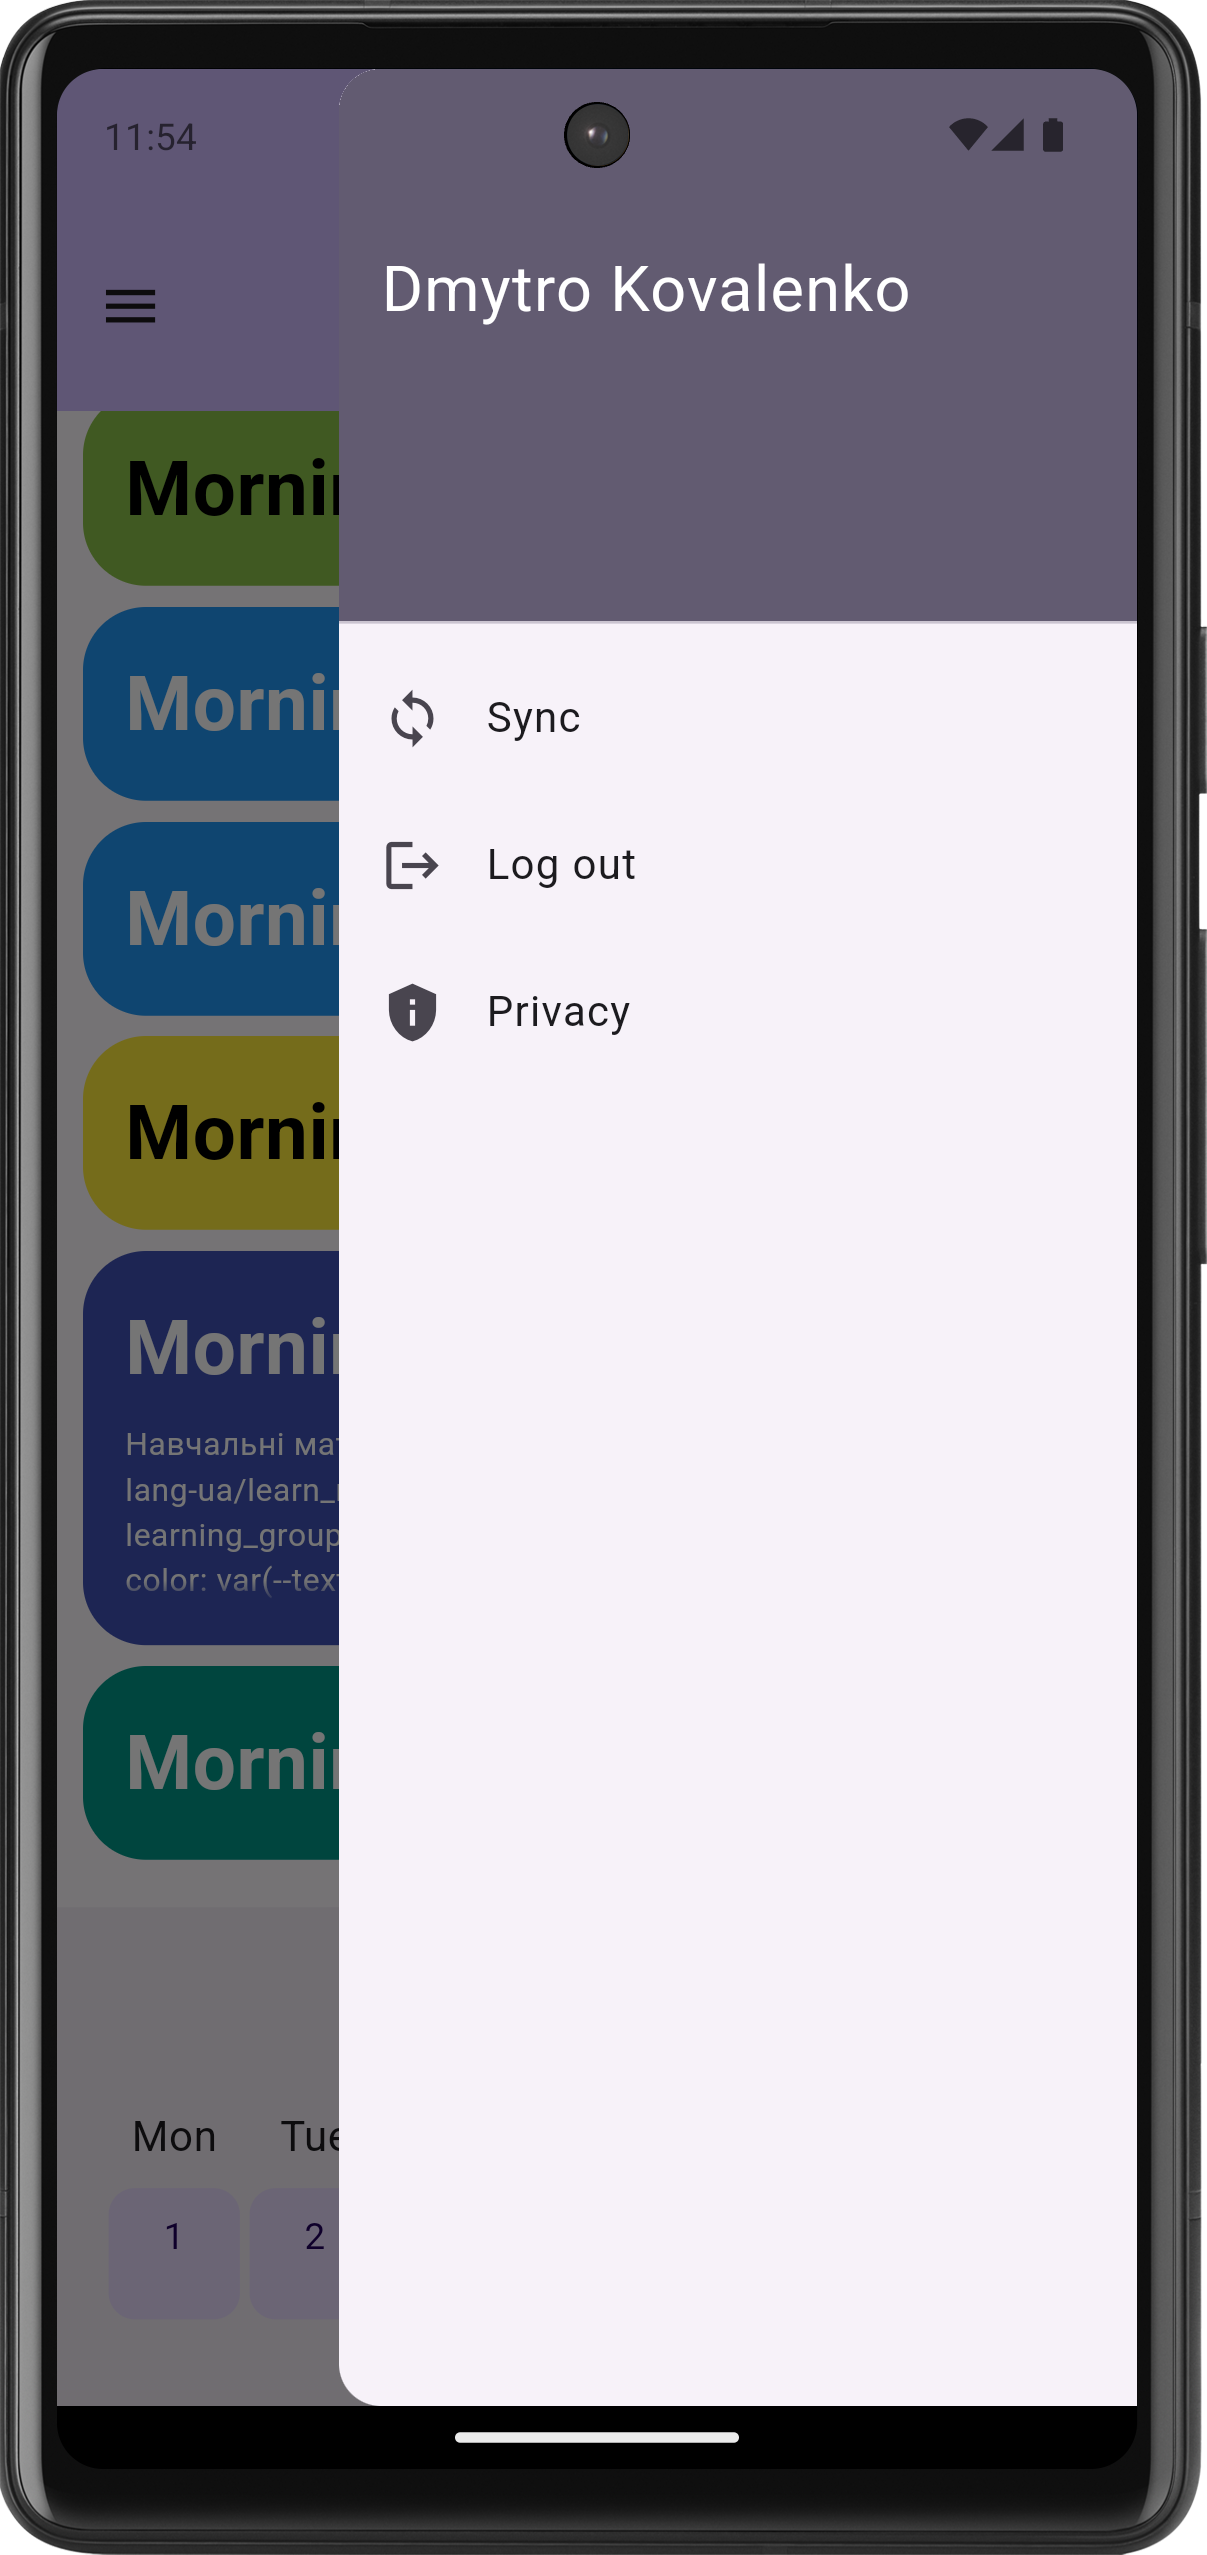
\includegraphics[scale=0.12]{8}
			\caption{Можливість синхронізації подій з Google Calendar}
		\end{minipage}
	\end{figure}
	
	\section*{Висновки}
	Під час виконання лабораторної роботи я розробив мобільний застосунок згідно з обраним варіантом.
	    
\end{normalsize}
\end{document}
